\chapter{Introducing Power Compensations}
\label{cha:power_compensations}

\minitoc

\section{Introduction}

In this chapter, we propose some heuristics to solve the problem from the model presented in Section \ref{sec:ODM}. Due to the uncertainties, online scheduling needs to adapt the offline plan. To address this, we propose two contributions in this chapter. First, we schedule the jobs according to the power envelope. The second contribution is to adapt the power envelope, using power compensations. Power compensations are modifications in the power envelope to approximate the battery SoC at the end of the time window to the offline plan. First, we describe the heuristics to solve it, linking with the model from Chapter \ref{cha:model}. This heuristic includes scheduling and power decisions. Then, we explain the experimental environment used in the experiments. Finally, we present and discuss the results, highlighting the impact of the power constraints.

\section{Proposed Approach}

We divided the heuristic into two parts. First, we detail the scheduling decisions. The scheduler defines the job priority and placement. The main objective of the scheduling is to finish the jobs, avoiding killing them. To do so, the scheduler can demand more power, adapting the power envelope. Then, we describe the power compensation heuristics. Power compensations are modifications in the power envelope (given by the offline side). These modifications are needed because the real power production and demand can vary from the offline, due to the uncertainties. The power compensations' objective is to approximate the battery's state of charge from the target level at the end of the time window. Finally, the scheduler must translate the power modifications into server configurations. We explain our heuristic to do it.

\subsection{Scheduling}
\label{sec:heuristic_scheduling}

Job scheduling is a well-known problem NP-complete problem \cite{robert2009introduction, agrawal2021energy}. Several heuristics are proposed to solve this problem in an acceptable time. We implemented and adapted a well-known algorithm named EASY Backfilling in this chapter for the job placement \cite{mu2001utilization}. This heuristic is known for its simple and robust implementation \cite{srinivasan2002characterization}. Furthermore, it maximizes server utilization \cite{srinivasan2002characterization}. EASY backfilling focuses on job placement, but the scheduler also adapts the power envelope to avoid killing jobs. The placement heuristic runs on every job arrival, job finished, and new time step. On the other hand, the power envelope adaptation runs at each new time step only. First, we present the placement algorithm. This algorithm englobes queue sorting and placement. First, it places priority jobs in the available servers. Then, it fills the scheduling holes with small jobs (see Figure \ref{fig:backfilling}). Algorithm \ref{alg:algo_scheduling} denotes a pseudo-code of EASY Backfilling, presented by \citeauthor{lelong2018tuning} as EASY-$P_{R}$-$P_{B}$ policy \cite{lelong2018tuning}.

\IncMargin{1em}
\begin{algorithm}[!htb]
    \LinesNumbered
    \footnotesize
    \SetAlgoLined
    \SetKwInOut{Input}{input}\SetKwInOut{Output}{output}
    \Input{Queue $Q$ of waiting jobs, $P_{R}$ as priority order, and $P_{B}$ as backfilling order.}
    \Output{None (calls to \textit{Start()})}
    \Begin{
        Sort $Q$ according to $P_{R}$\;
        \For{job $j$ in $Q$}{
            Pop $j$ from $Q$\;
            $S_j \leftarrow$ \textit{select\_servers($j$)}\;
            \uIf{$j$ can be started in servers $S_j$}{
                \textit{Start($j$, $S_j$)}\;
            }\Else{
                Reserve $j$ at the earliest time possible according to the walltime of the currently running jobs\;
                Sort $Q$ according to $P_{B}$\;
                \For{job $j^{'}$ in $Q$}{
                    $S_j \leftarrow$ \textit{select\_servers($j^{'}$)}\;
                    \If{$j^{'}$ can be started in servers $S_j$ without delaying the reservation on $j$}{
                        \textit{Start($j^{'}$, $S_j$)}\;
                    }
                }
                \textbf{break}\;
            }
        }
    }
    \caption[EASY-$P_{R}$-$P_{B}$ scheduling.]{EASY-$P_{R}$-$P_{B}$ scheduling \cite{lelong2018tuning}.}
    \label{alg:algo_scheduling}
\end{algorithm}
\DecMargin{1em}

First, this heuristic sorts the jobs in the queue in a priority order $P_{R}$ (line 2). Then, it selects the servers to run this job (line 5). If the job $j$ can start in the servers $S_j$ (line 6), it places the job in the servers (line 7). When it finds a job that can not start now, the algorithm starts to backfill (lines 9-17). Then, it reserves the first moment to run this job (named priority job) in the future (line 9). So, it re-sorts the queue using $P_{B}$ (line 10), placing the other jobs in the servers (lines 11-16) without delaying the (future) priority job execution (line 13). As presented, the algorithm sorts the queue using $P_{R}$ (in the priority moment) and $P_{B}$ (in the backfilling moment). However, the typical implementation uses the same sort for both \cite{lelong2018tuning}. Our first implementation uses the typical algorithm (same sorting policy). Thus, $P_{R}$ and $P_{B}$ apply the Descending Bounded Slowdown (higher Bounded Slowdown first) policy from Equation \ref{equ:slowdown}. This order helps to let a job wait proportionately to its size.

Besides the placement, the scheduler makes power envelope adaptations to maintain the jobs running at least at a "minimal speed". These decisions occur at each new time step. This minimal speed is given by Equation \ref{equ:avoid_walltime}. The idea is to keep the jobs' servers at the speed $D_{s,d}$ (it is the DVFS speed). For example, if $D_{s,d}$ is too slow, the job can reach the walltime without finishing all its computing. Besides, if a server goes to sleep, its running jobs are killed. So, every time step $t$, the scheduler verifies the energy needed to maintain the jobs running at least at minimal speed. If it is necessary to use more energy now (changing the plan), it verifies if it is possible to migrate power from the future to now. This verification consists of two tests:
\begin{enumerate}
    % \item \textit{Does the battery have the energy to be migrated?} The algorithm calculates how much battery energy is planned to be used in the future. The algorithm must let minimal energy to maintain all servers in the sleep state (it can come from battery, renewable, or hydrogen). So, the energy needed to maintain jobs running must be present in the sum of future usage;
    % In this test, the algorithm verifies the battery usage in future steps. Let $P_{min}$ be the power needed to maintain all servers in the sleeping state. So, for each step, the energy possible to migrate from the batteries is equal to:
    % \begin{itemize}
        %     \item If $P_{fc} > P_{min}$: $P_{renew} + P_{dch} - P_{ch}$. In this case, hydrogen maintains the servers in the sleeping state. So all renewable can be used to charge the battery;
        %     \item If not: $P_{renew} + P_{dch} - P_{ch} - P_{ez} - P_{min}$
        % \end{itemize}
    \item \textit{Will battery boundaries be violated?} Equation \ref{equ:battery_boundaries} must be respected. So, migration can not violate the SoC boundaries;
    \item \textit{Is it possible to compensate for this change?} Section \ref{sec:power_compensation} explained this verification;
\end{enumerate}

If possible, the scheduler modifies the offline IT plan to let the servers run at P-state $D_{s,d}$. If not, the scheduler does not change the offline plan.

\subsection{Power compensations}
\label{sec:power_compensation}

After describing the scheduling algorithm, this section explains the heuristic to compensate for power fluctuations presented in Section \ref{sec:ODM}. The power compensations' objective is to ensure that $SoC$ and $LoH$ are close to the offline plan at the end of the time window. Therefore, every time step $t$, ODM calculates $E_{comp}$ using Equation \ref{equ:energy_battery}. As explained in Chapter \ref{cha:model}, we can have two kinds of compensations: positive and negative. So, $E_{comp}$ can be positive or negative, according to battery usage or renewable production. A positive compensation indicates that the scheduler can use more energy to run jobs. On the other hand, negative compensation demands a reduction in usage to finish the time window close to the battery target level. Thus, the problem is to define the future time step to use energy $E_{comp}$. Let $t'$ be the future time step. Then, ODM must change $P_{dch}(t')$ and $P_{ch}(t')$. Of course, $P_{dch}$ and $P_{ch}$ are power, and $E_{comp}$ is energy, so we adapt to work only with energy in this process. Furthermore, the changes must consider the boundaries from Equations \ref{equ:discharge_boundary} and \ref{equ:charge_boundary}. In addition, the power usage in the sleep state is not zero, demanding minimal power production. Let $P_{min}$ be the minimal power possible. Then, $P_{prod}(t') \ge P_{min}$, considering that $P_{prod}$ comes from Equation \ref{equ:model_energy}. 

ODM spreads the energy over different $t'$ until all modifications compensate for $E_{comp}$. The power compensations happen in two cases:
\begin{itemize}[leftmargin=.6in]
    \item[Case 1] Every time step, ODM recalculates $SoC(T)$ using Equation \ref{equ:battery_energy} from the actual step until $T$. Then, it compares $SoC(T)$ and $SoC_{target}$, using Equation \ref{equ:delta_energy}. Finally, ODM compensates $E_{comp}$ (from Equation \ref{equ:energy_battery}), approximating $SoC(T)$ to $SoC_{target}$ (respecting Equation \ref{equ:soc_target});
    \item[Case 2] When the scheduler demands more power, as presented in Section \ref{sec:heuristic_scheduling}, it tries to maintain the servers with jobs running. So, it increases the power usage at the step. This increase will change the $SoC(T)$, demanding compensation. This compensation is always negative (if ODM uses more power now, it reduces the usage in the future).
\end{itemize}

If ODM can not entirely compensate $E_{comp}$, it has two possible actions. If the request for compensation comes from the scheduler (case 2), it does not make the modifications demanded by the scheduler, impacting the jobs. On the other hand, in case 1, ODM will modify as much as possible. On Datazero2, the impossibility of compensating for case 1 can start a new negotiation from the offline part to deal with this event. However, in this thesis, we let the simulation run to see the impact of these cases, resulting in a SoC difference at the end of the time window.

The question now is: in which future time step $t'$ can we compensate? To answer this question, we propose four policies: \emph{Peak}, \emph{Next}, \emph{Last}, and \emph{Load}. Figure \ref{fig:compensation} illustrates an example of these policies. The \emph{Next} and \emph{Last} policies execute the same search independently of the type of compensation (positive or negative). While \emph{Next} takes the $t + 1$, \emph{Last} takes $T$. On the other hand, \emph{Peak} and \emph{Load} take different steps according to the compensation (positive or negative). \emph{Peak} policy finds the higher power production ($P_{prod}$) peak in negative compensation and the lower peak in positive. This policy will "shave" the peaks, tending to a flat curve. \emph{Load} policy considers the difference between demand ($P_{load}$) and production ($P_{prod}$). In positive compensation, this policy takes the higher difference $P_{load} - P_{prod}$, while in negative it takes the smaller one. In Figure \ref{fig:compensation}, if the scheduler saves energy at step 1, it could compensate for it at step 3 (\emph{Next}), step 12 (\emph{Peak}), step 15 (\emph{Last}), or step 14 (\emph{Load}). Even if Figure \ref{fig:compensation} compensates only one time, the algorithm can select more than one, compensating $E_{comp}$ entirely and following its policy (e.g., \emph{Next} will take steps 2, 3, 4, etc.).

\begin{figure}[!htb]
    \centering
    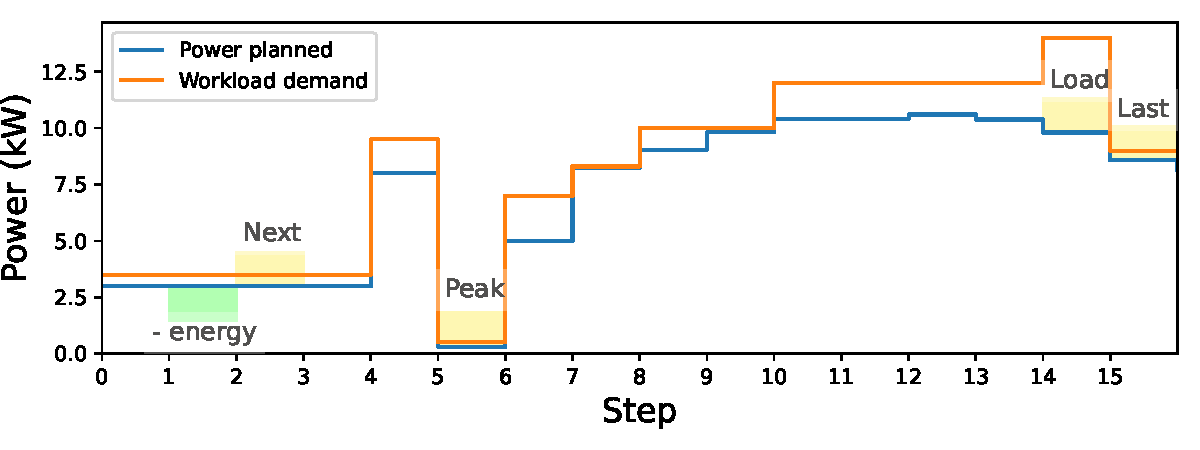
\includegraphics[scale=0.7]{Images/Compensations/policies.pdf}
    \caption[Compensation policies]{Compensation policies. This is an example of positive compensation (it uses less energy at step, so we need to increase the usage in the future). The blue curve is the offline usage plan ($P_{prod}$) and the orange line is the estimated demand ($P_{load}$). In this example, it saves some energy in time step 1 (see the green square). So, it can reintroduce this energy in future time steps (see the yellow squares).}
    \label{fig:compensation}
\end{figure}

\subsection{Server configuration}
\label{sec:server_configuration}

Finally, the last part of the heuristic is transforming the power modifications into server configuration. Since the IT offline plan gives the P-state of the servers for each step $t$, we must adapt this plan for the new power. We propose a heuristic to find quick solutions. The four policies use the same heuristic to distribute the compensation. This heuristic has a list of all power and speed differences between two P-states, so it can fastly decide which one will impact the most on data center speed. First, it calculates the difference between the power usage in the offline plan and the power to use. If this difference is positive, it can improve the server configuration, speeding up or turning on servers. It searches on the list for the highest flops improvement below or equal to the power increment. It does it in the following order:
\begin{enumerate}
    \item Find the highest improvement possible for the servers running some job;
    \item Find the highest improvement possible for the servers not running jobs.
\end{enumerate}

Taking Table~\ref{tab:gros} as an example, let's say that we have two servers running jobs: one on state 5 and another on state 10. The system has 30 W to increase. So, it will increase first the server on state 10 to state 1, because it will increase 14.41 Gflops (against 6.45 Gflops from state 5 to state 1). If a server is sleeping, it also considers the power needed to turn the server on. When the difference between offline and online power is negative, the algorithm must reduce the speed of the servers. So, it does the following:
\begin{enumerate}
    \item Reduce the speed of servers not running jobs;
    \item We calculate $(wall_{j} - elapTime_{j})$ for each job running. Then, we sort the servers by this value in decreasing order. Finally, we reduce the speed of these servers following this order. 
\end{enumerate}

It stops after the first modification that lets the power usage lower or equal to the power production $P_{prod}(t)$. The second step will reduce servers' speed with more time to compensate for this reduction in the future. It is better to maintain jobs closer to finish with the maximum speed, granting that they will be complete.

\section{Experimental environment}
\label{sec:experiment_environment}
% IT (servers)
% Electrical (battery, solar, wind, etc)
% Workload Trace
% Weather Trace

In this section, we present the environment used to run our simulations. This environment englobes IT servers definition, electrical elements, workload trace, and weather trace. We focus on simulating a time window of three days ($T_{w}=259200 s$), divided into time steps of 5 minutes ($\Delta t=300$). We chose time steps of 5 minutes because it is neither too long to react to events nor too short for server transitions. For example, a time step of 1 minute is a good choice for adapting the battery usage, but it is not enough to turn on a server (Table \ref{tab:gros} shows that a Gros server takes 164 seconds to finish the off$\rightarrow$on transition). A longer time step can be too late to adapt battery usage. Concerning the server specification, we simulated a homogeneous data center using the GRID5000's Gros server. Table \ref{tab:gros} presents their parameters. We demonstrate the experiments in a homogeneous data center to ease the understanding. However, we proposed different experiments in a heterogeneous data center in \cite{de2022analyzing}. Our data center is composed of 400 servers with Gros specifications. We ignored other aspects, such as network and memory. 

Considering the electrical components, the data center is composed of solar panels, wind turbines, batteries, and one hydrogen tank. The total size of the batteries is 800 kWh ($C_{bat}=800kWh$). The efficiency of charging is 0.82 ($\eta_{ch}=0.82$), and discharging is 0.82 ($\eta_{dch}=0.82$). We defined the thresholds $SoC_{min}$ and $SoC_{max}$ as 20\% and 90\%. So, the battery energy range maintains the whole data center for 9.76 hours. We set the max charge and discharge power as 80\% of the battery size ($P_{ch_{max}}=640kW$ and $P_{dch_{max}}=640kW$). The hydrogen tank has 20000 kg ($LoH_{max}=20000$).
%  with the electrolyzer's efficiency of 97.5 and the fuel cell's efficiency of 13.332. 
At the beginning of the experiment, the battery starts half charged ($SoC(0)=50\%$) and the hydrogen with 300 kg ($LoH(0)=300kg$). We also specified that they should return at least to the same value as they started at the end of the time window ($SoC_{target} = 50\%$ and $LoH_{target}=300kg$).

We have divided the experiments into two parts that use different weather and workload traces. The first part analyzes the decisions in critical cases (named \emph{critical scenarios}), and the second part focuses on the random cases (named \emph{random scenarios}). 

\subsection{Critical Scenarios}

In the first part, we have taken two workloads from the Metracentrum dataset with the size of three days. The first workload has jobs arriving mainly on the first day and the second one on the third day. Figure \ref{fig:critical_workload} illustrates the demanded power of both workloads. We calculated this power using 400 Gros servers without power constraints (e.g., the servers are always available). The first workload has 3729 jobs and the second workload has 3158 jobs. Even if the second one has fewer jobs, it is more complicated to manage since the jobs arrive on the last day.

\begin{figure}[!htb]
    \centering
    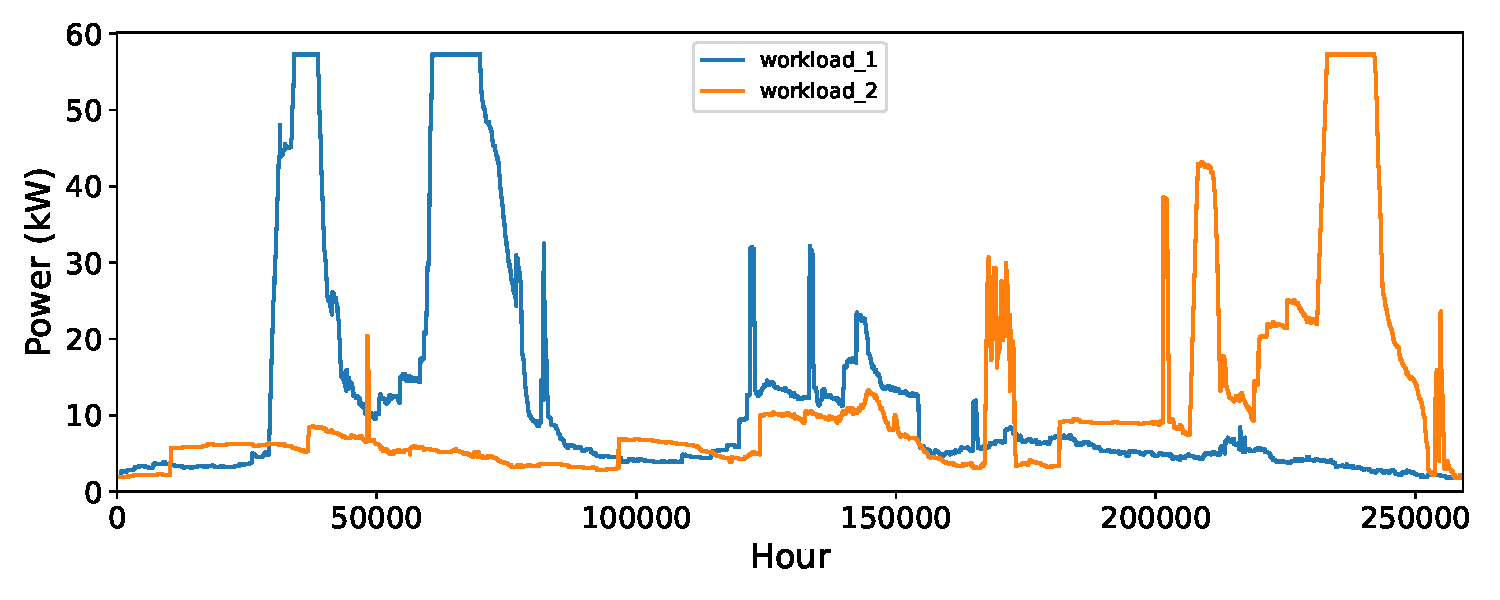
\includegraphics[scale=0.58]{Images/Compensations/critical_jobs_arriving.pdf}
    \caption{The power demanded for the critical scenarios.}
    \label{fig:critical_workload}
\end{figure}

We generated the three-day weather data using MERRA and renewable ninja for the critical scenarios \cite{rienecker2011merra, pfenninger2016long, staffell2016using}. Figure \ref{fig:critical_weather} shows the power production generated by the weather using the electrical components of our data center. 

\begin{figure}[!htb]
    \centering
    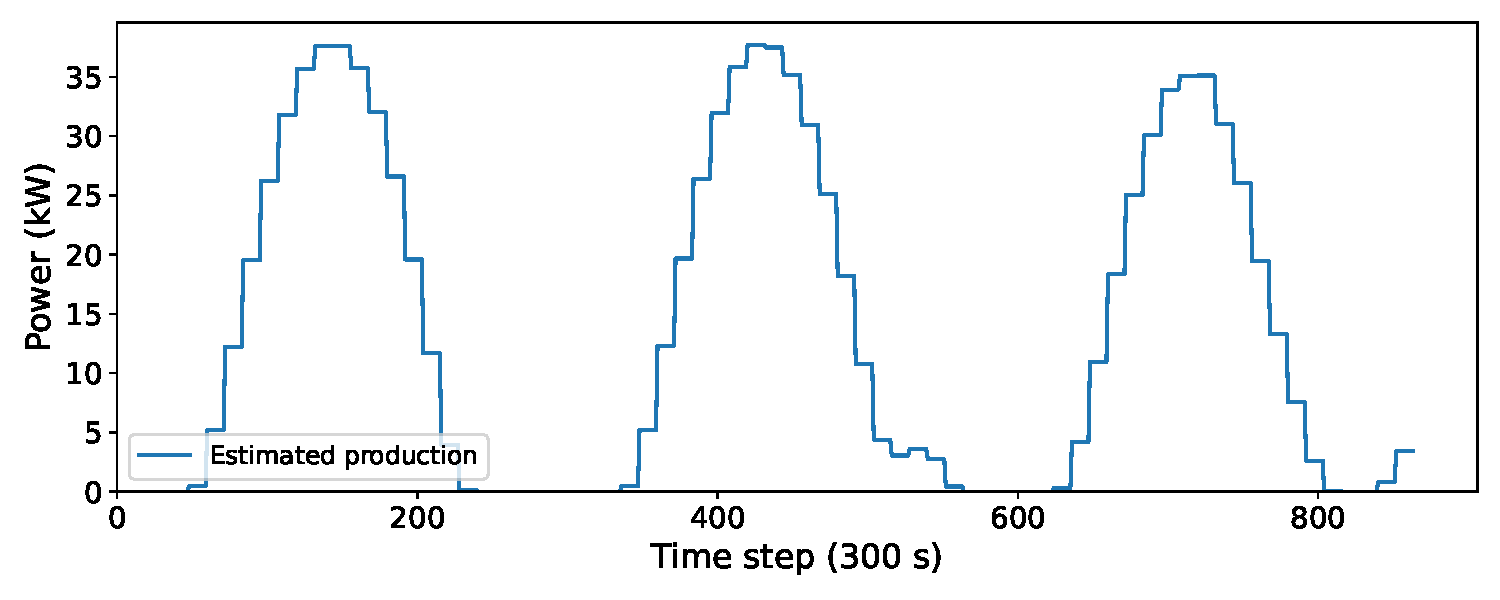
\includegraphics[scale=0.58]{Images/Compensations/critical_power_production.pdf}
    \caption{The power production for the critical scenarios.}
    \label{fig:critical_weather}
\end{figure}

We consider both workload and weather as predictions. Then, we use them to create the offline plan from Section \ref{sec:offline_plan}. First, we solved the PDM model from Section \ref{sec:offline_modules} using the linearization proposed by \citeauthor{haddad2019mixed} \cite{haddad2019mixed}. Then, we took the production ($P_{prod}$) and solved the ITDM model. The ITDM model presented in Section \ref{sec:offline_modules} is too complex to solve a three-day time window with 400 servers. So, we simplified the problem, ignoring the transitions on$\rightarrow$off and off$\rightarrow$on. This new model returns the number of servers at each P-state at each time step and can be solved faster. After that, we have the offline plan. 

The next step is to introduce noise in the predictions to emulate the variations in reality. Every prediction provides a range of where the forecast is likely to be. So, we generated noises inside this range. In the critical scenarios, we considered that the range is $\pm 20\%$. Then, we created two new power productions: a worst-case and a best-case. In the worst-case scenario, all the productions are 20\% lower than predicted. On the other hand, in the best-case power production, all productions are 20\% higher. Figure \ref{fig:critical_weather_with_noise} illustrates the power production. Therefore, we simulated the worst and best cases of production (the reason for the name critical scenarios).

\begin{figure}[!htb]
    \centering
    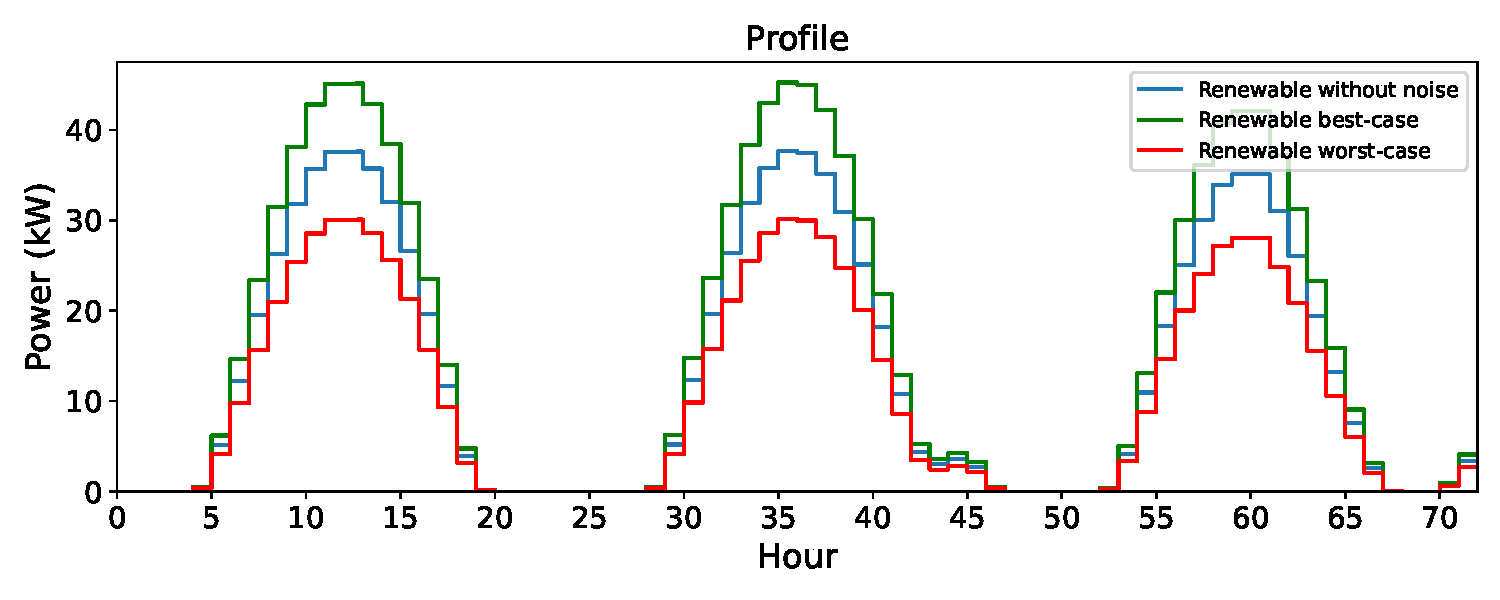
\includegraphics[scale=0.58]{Images/Compensations/critical_power_production_with_noise.pdf}
    \caption{The power production with noise for the critical scenarios.}
    \label{fig:critical_weather_with_noise}
\end{figure}

Regarding the workload, we introduced Gaussian noises in interarrival and job duration with a standard deviation of 20\% of the predicted value. The relation between these workload noises and the power demand is more complicated than the power production since the power demand depends on the scheduling algorithm and queue sort. Figure \ref{fig:critical_workload_with_noise} shows the impact of these noises on the power demand. Even if the impact on the workload power demand is not huge, these variances impact the offline IT plan since offline can indicate the wrong moment to turn on/off the servers. The workload's criticality comes from when the jobs arrive (in the end or beginning).

\begin{figure}[!htb]
    \centering
    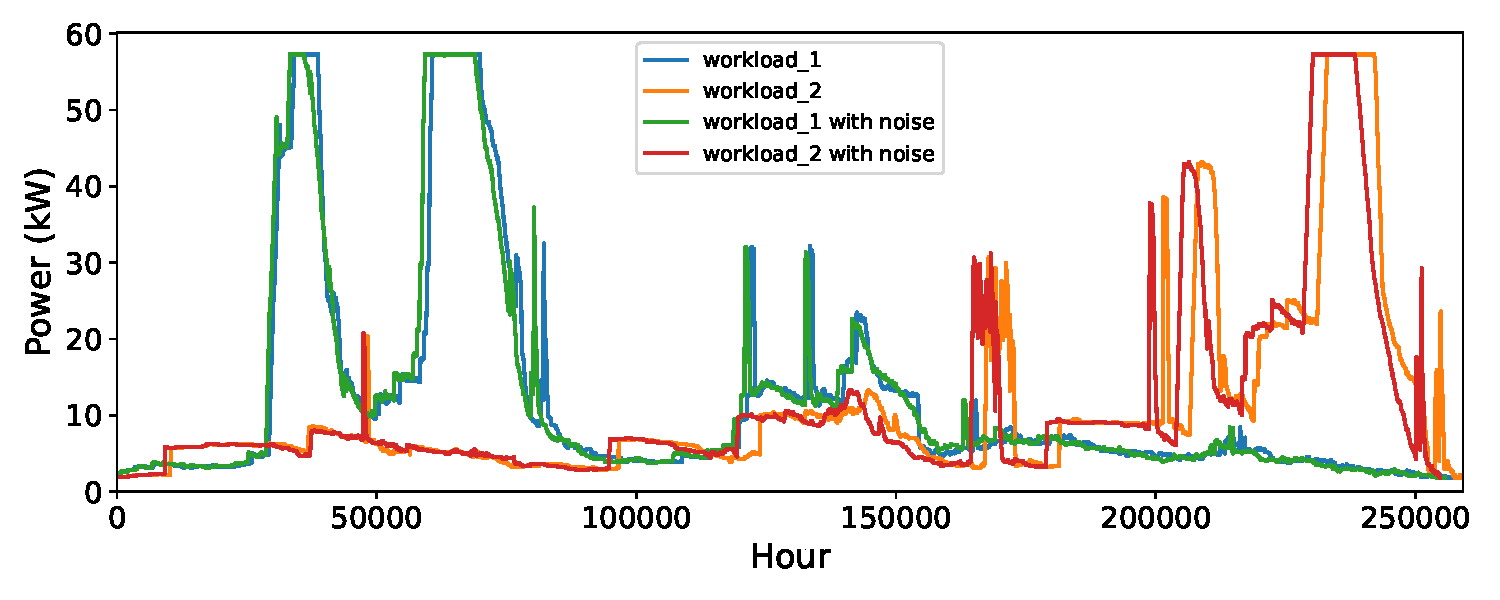
\includegraphics[scale=0.58]{Images/Compensations/critical_jobs_arriving_with_noise.pdf}
    \caption{The power demand with noise for the critical scenarios.}
    \label{fig:critical_workload_with_noise}
\end{figure}

Finally, we mixed the two productions (worst and best-case) with the two workloads (in the end and beginning), creating four scenarios:

\begin{enumerate}
    \item \emph{Critical 1}: Profile best-case and workload in the beginning;
    \item \emph{Critical 2}: Profile best-case and workload in the end;
    \item \emph{Critical 3}: Profile worst-case and workload in the beginning;
    \item \emph{Critical 4}: Profile worst-case and workload in the end;
\end{enumerate}

The first scenario is the best possible, with more energy and having all the jobs in the beginning. Therefore, the scheduler has the energy and time to decide when to place the jobs. However, the last scenario is more complicated, with lower production and receiving the jobs on the third day.

\subsection{Random Scenarios}

In the \emph{Random Scenarios}, we generated ten workload and weather traces. Figures \ref{fig:average_weather_with_noise} and \ref{fig:average_workload_with_noise} show the power production and demand, respectively. Then, we created ten offline plans, one for each pair of workload and profile. For example, workload 1 receives the production of profile 1, workload 2 receives profile 2, etc. We created the offline plans in the same way as the critical cases for each combination.

\begin{figure}[!htb]
    \centering
    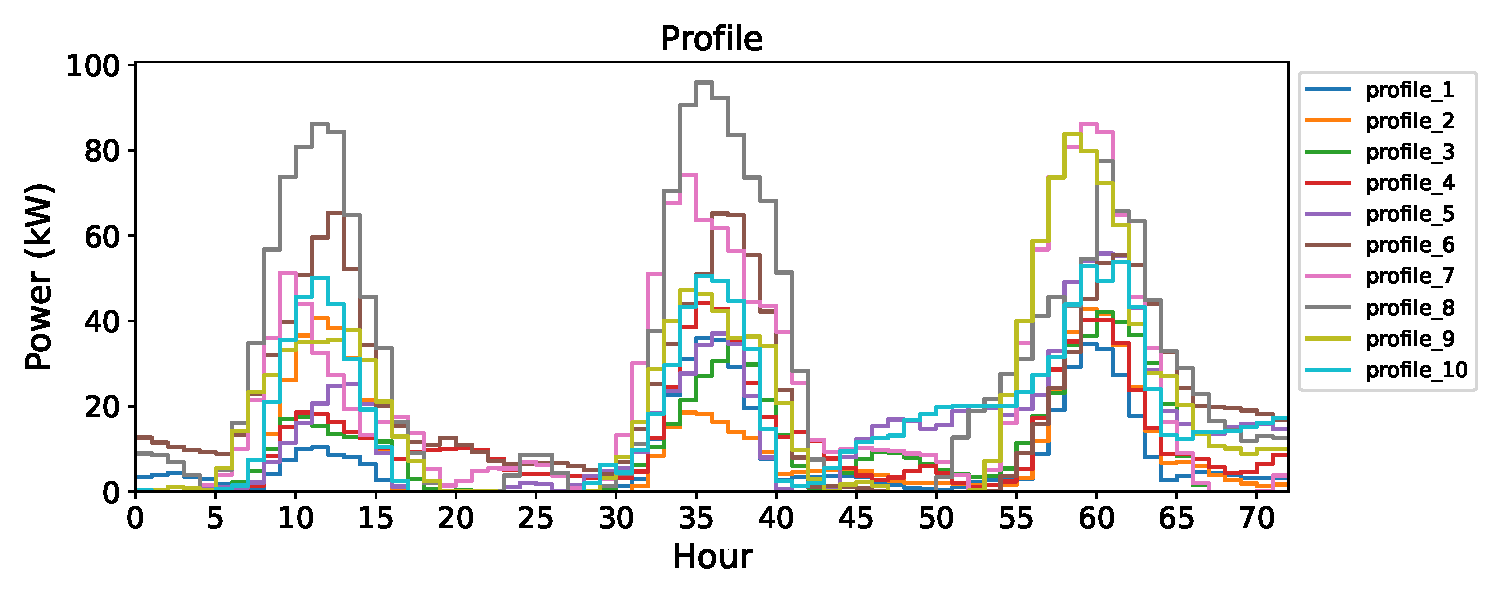
\includegraphics[scale=0.58]{Images/Compensations/diff_power_production.pdf}
    \caption{The power production for the random scenarios.}
    \label{fig:average_weather_with_noise}
\end{figure}

\begin{figure}[!htb]
    \centering
    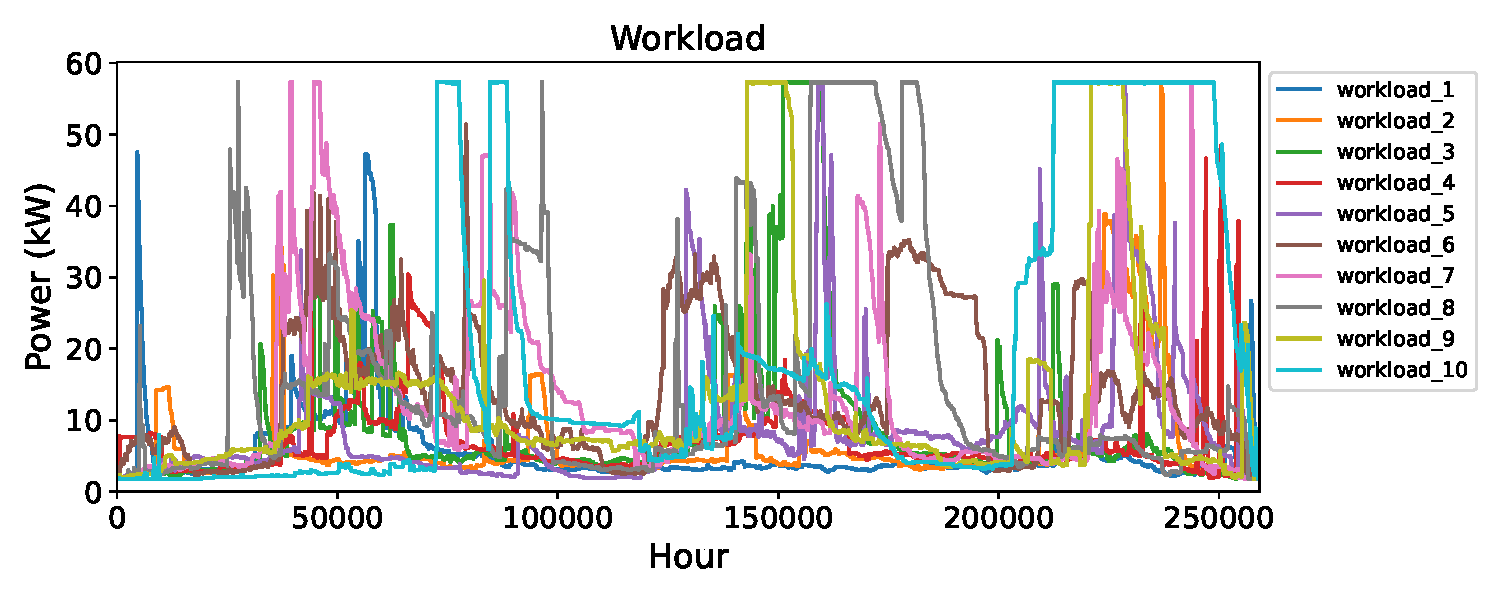
\includegraphics[scale=0.58]{Images/Compensations/diff_jobs_arriving.pdf}
    \caption{The power production for the random scenarios.}
    \label{fig:average_workload_with_noise}
\end{figure}

After creating the plans, we introduce noise in the values. Here, we applied Gaussian noises in power production and jobs interarrival and size. We increase the standard deviation to 50\%, giving a wider range to generate values. Therefore, we have higher uncertainty. For each pair (workload + profile), we produced ten new workloads and profiles with noise, resulting in 100 combinations. We called these scenarios \emph{Random Scenarios} because they are neither worst case nor best case. 

\textbf{In both parts (critical and random), besides the production and jobs noises, we also have the uncertainty from the walltime, presented in Section \ref{sec:workload_trace}.} So, our experiments introduce several uncertainties in different aspects of workload and power production. Furthermore, these uncertainties are cumulated from the different steps.

\subsection{Baselines}
We created three baselines to compare the results from the four policies. The baselines are \emph{Follow plan}, \emph{Power reactive}, and \emph{Workload reactive}. \emph{Follow plan} is an algorithm that applies the offline plan without changing it. This algorithm emulates the execution of only the offline side. \emph{Power reactive} changes the server state according to the renewable power incoming. So, at each time step, it takes the power coming from renewable and calculates how many servers are possible to maintain running. It uses power from the batteries to maintain jobs running, if the renewable is not enough. \emph{Power reactive} uses the server configuration heuristic presented in Section \ref{sec:server_configuration}. \emph{Workload reactive} turns on the servers according to the job's arrival. It starts with all servers off. For each new job submitted, it turns on the needed server at maximum speed if there is no server idle. After finishing a job, the server waits for $T_{wait}$ seconds (using the DPM technique from Equation \ref{equ:dpm_waiting_time}). The scheduler sedates the server if it stays idle for $T_{wait}$ seconds. In all cases (baselines and compensation policies), if the battery's state of charge arrives at less than 20\% (defined $SoC_{min}$), the scheduler kills the jobs and sedates all servers. 

\section{Results Evaluation}

After describing the experimental environment, this section presents the results of the experiments. We detail the critical and random scenarios. After that, we discuss the results globally.

\subsection{Critical cases}

\subsubsection{Scenario Critical 1}
Scenario Critical 1 (Profile best-case and workload in the beginning) has the jobs arriving at the beginning, and the production is higher than expected. However, this scenario is tricky. Since the battery starts with $SoC = 50\%$, if the scheduler starts too many jobs in the beginning, this can lead to a very low $SoC$ on the first day. This is exactly what happened with \emph{Workload reactive} in this scenario. Figure \ref{fig:DPM_soc} shows the evolution of the state of the charge in the \emph{Workload reactive} execution. At step 264 (79200 seconds after the simulation begins), \emph{Workload reactive} has less than 20\% of SoC. So, the scheduler kills several jobs. 

\begin{figure}[!htb]
    \centering
    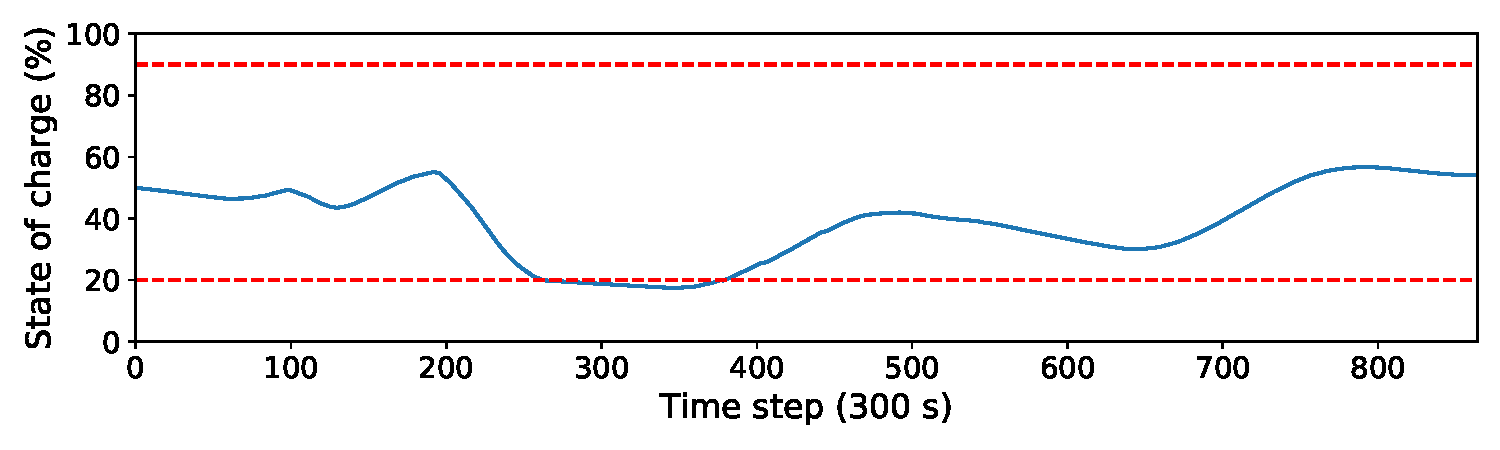
\includegraphics[scale=0.55]{Images/Compensations/critical_soc_s1.pdf}
    \caption{State of Charge for \emph{Workload reactive}.}
    \label{fig:DPM_soc}
\end{figure}

Figures \ref{fig:SoC_critical_1} and \ref{fig:jobs_critical_1} give the battery level at the end of the time window and jobs states, respectively. Figure \ref{fig:jobs_critical_1} shows two graphs. The first one considers only the number of jobs, ignoring their size. Therefore, all jobs are equal. In the second graph, we consider the size of the job. So, bigger jobs have more importance than smaller ones. The second graph illustrates the mass of work to do.

\begin{figure}[!htb]
    \centering
    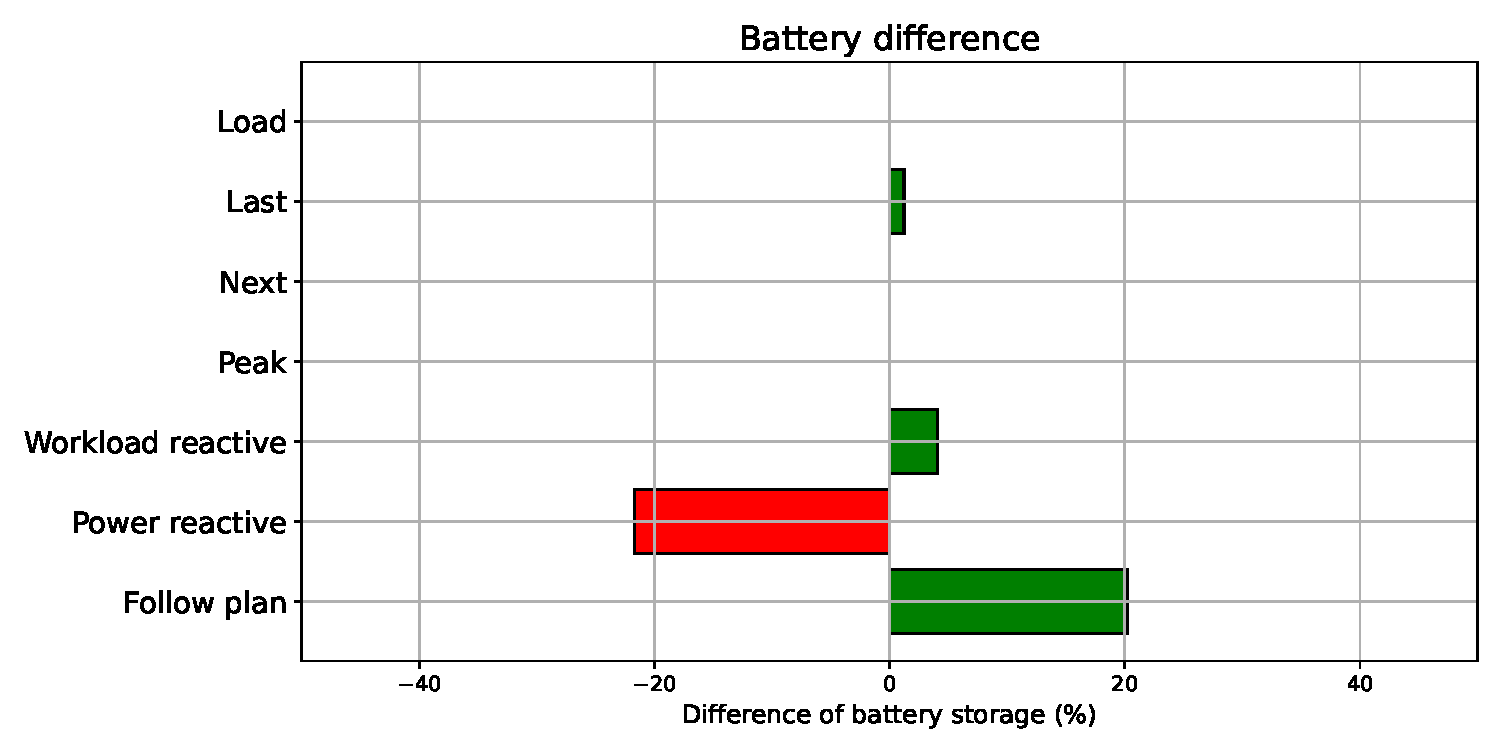
\includegraphics[scale=0.55]{Images/Compensations/battery_critical_1.pdf}
    \caption{Difference between the battery target level (50\%) and the real battery level at the end of the time window for scenario critical 1.}
    \label{fig:SoC_critical_1}
\end{figure}

\begin{figure}[!htb]
    \centering
    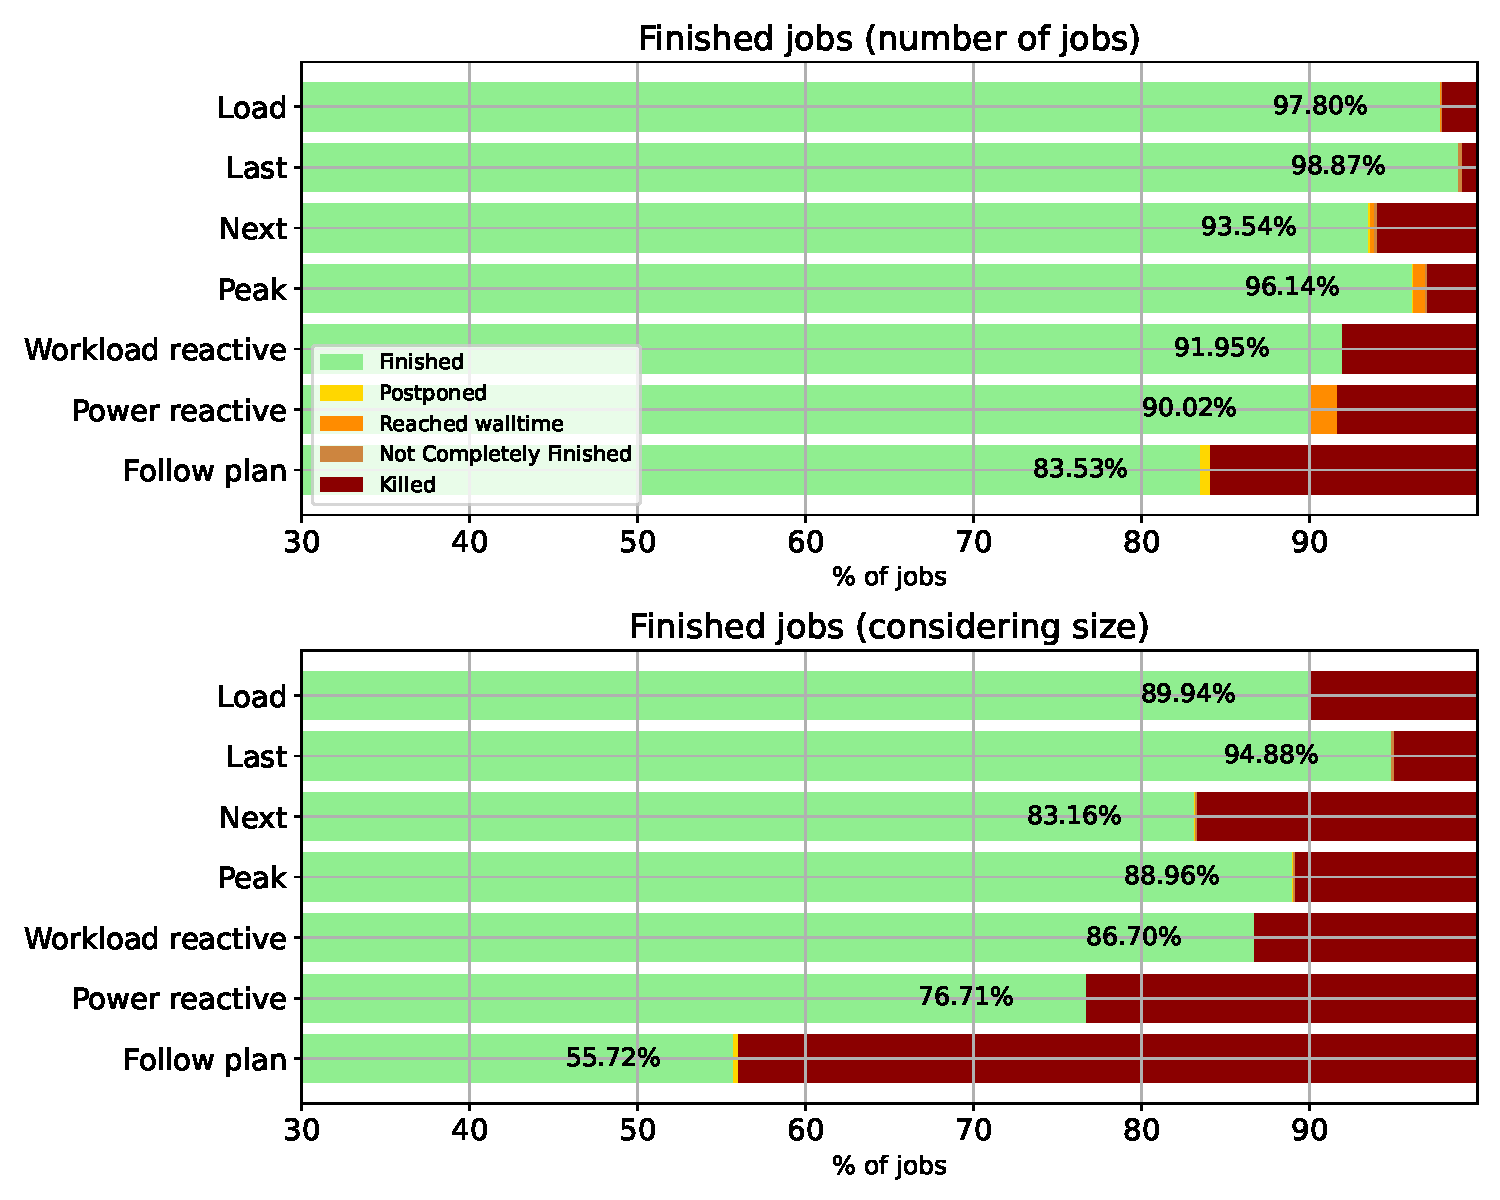
\includegraphics[scale=0.55]{Images/Compensations/jobs_critical_1.pdf}
    \caption{Jobs states at scenario critical 1. The first graph (above) considers only the number of jobs, ignoring their size. In the second graph (below), the jobs' size is considered.}
    \label{fig:jobs_critical_1}
\end{figure}

It is important to analyze the battery level and finished jobs together. For example, \emph{Follow plan} saves energy, finishing with 20\% more battery than the target. This result seems very good, but analyzing Figure \ref{fig:jobs_critical_1}, \emph{Follow plan} has the lower finished jobs and higher killed jobs. Besides, it kills a lot of big jobs, resulting in only 55.72\% of finished jobs considering the size. This result illustrates the importance of reacting to real events and using the saved energy to improve QoS. \emph{Follow plan} tends to kill bigger jobs since it does not adapt the plan to maintain them running.

\emph{Power reactive} has the worst battery level, with an SoC of around 28\% (difference of -21.729269\%). This algorithm allocates all incoming power from renewable sources to servers, not recharging the battery. The battery slightly recharges due to power fluctuations (e.g., the server is idle, so the incoming renewable power recharges the battery instead of going to the server). So, \emph{Power reactive} uses the battery to avoid killing jobs, but it does not compensate for this change. \emph{Power reactive} is the second-worst finished jobs metric (ignoring or considering the size), with some jobs reaching the walltime. Since it only uses the battery to avoid killing jobs, sometimes it let the servers at slower speeds, increasing the possibility of reaching walltime. It also kills some jobs because it also reaches the $SoC_{min}$.

As mentioned at the beginning of this section, \emph{Workload reactive} can not manage well the state of charge, killing some jobs. Even so, it finishes with a good battery level. The DPM technique helps to save some energy, letting the incoming renewable to recharge the battery. Since it always put the servers at maximum speed, no job reached the walltime. It has the third-worst finished and killed jobs (ignoring the size). All the policies are very close to the target level. Just \emph{Last} saved more than the target because it puts all the compensations in the end. Therefore, \emph{Last} can not use all the power before the end. Considering the metrics about the job, all policies finished more jobs and killed less than the three baselines. The best one is \emph{Last} with 98.87\% of the finished jobs considering the number of jobs and 94.88\% considering the size. In addition, it has the lowest killed jobs. \emph{Load} places the compensations in the steps where it expects high demand. In this case, it is worth it with the second-best results. We will see in future cases that this behavior is dangerous. 

\emph{Next} has the worst job result among the policies. It also kills more big jobs than the other policies and \emph{Workload reactive}. This result can be explained by comparing \emph{Next} and \emph{Last}. For example, let's say we saved energy in step 0. So, \emph{Last} increase the usage in the last possible step. If at any moment between step 0 and the last step, it is necessary to increase the usage, \emph{Last} can migrate the energy from the end and use it now. On the other hand, \emph{Next} expended this energy as soon as possible. Therefore, \emph{Next} can arrive in some moments without energy to avoid killing jobs. Finally, \emph{Peak} has the third-best result, with some jobs reaching the walltime. Since it shaves the power usage (negative/positive) peaks, it can reduce speed in critical moments (e.g., with several jobs running). However, it can maintain the big jobs running. Even if \emph{Peak} finishes fewer jobs than \emph{Load} (a difference of 1.66 percentage points), \emph{Peak} approximates the finished jobs considering the size (a difference of 0.98 percentage points).

The second analysis is regarding wasted energy. This metric is the energy expended not computing finished jobs, englobing, for example, the energy used in killed jobs, turning on/off servers, and letting servers idle. Figure \ref{fig:energy_critical_1} shows the results. \emph{Workload reactive} turns on resources on demand and does not let idle servers available too much. Therefore, it has the best wasted energy metric compared with the other algorithms. The worst case is \emph{Power reactive} which turns on servers according to the power available, not the demand. \emph{Follow plan} and the four policies are guided by the offline plan. Therefore, the noise introduced in the real workload can lead to some mismatch between demand and production. Since \emph{Follow plan} kills more jobs than the policies, this metric is higher for this algorithm. The energy expended in killed jobs is wasted since the result of the killed job is useless. \emph{Last} has the second-best wasted energy since it runs more jobs than the other algorithms.

\begin{figure}[!htb]
    \centering
    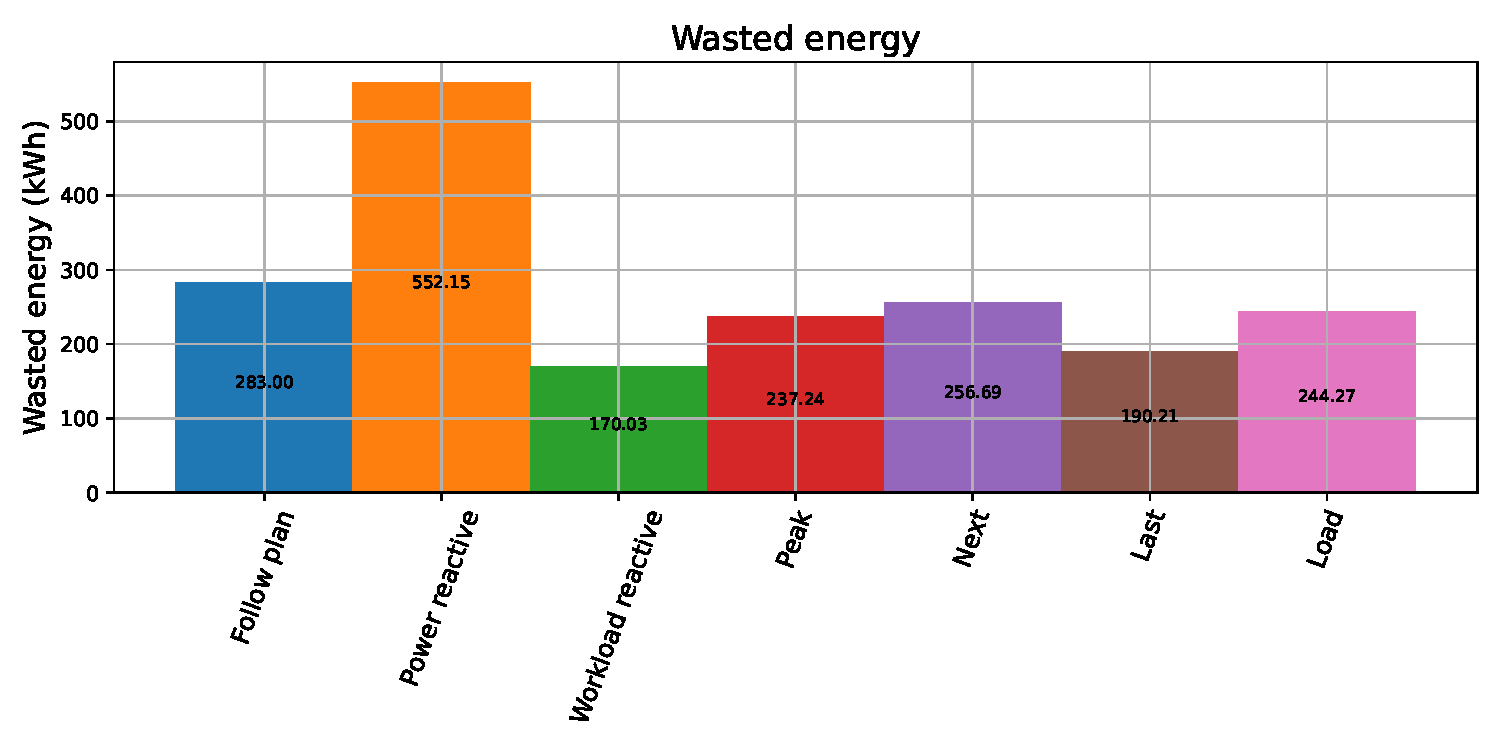
\includegraphics[scale=0.55]{Images/Compensations/energy_critical_1.pdf}
    \caption{Wasted energy at scenario critical 1.}
    \label{fig:energy_critical_1}
\end{figure}

Finally, Figure \ref{fig:slowdown_critical_1} demonstrates the slowdown of the finished jobs. As mentioned before, this metric is complicated to compare with different numbers of finished jobs. We can see that \emph{Workload reactive} has some jobs with a very high slowdown. It happens due to the long period with the SoC below $SoC_{min}$ (as illustrated in Figure \ref{fig:DPM_soc}). So, it has a long period without servers running. \emph{Load} has a good mean and median. In this case, \emph{Load} can place the compensations close to the jobs' arrival. 

\begin{figure}[!htb]
    \centering
    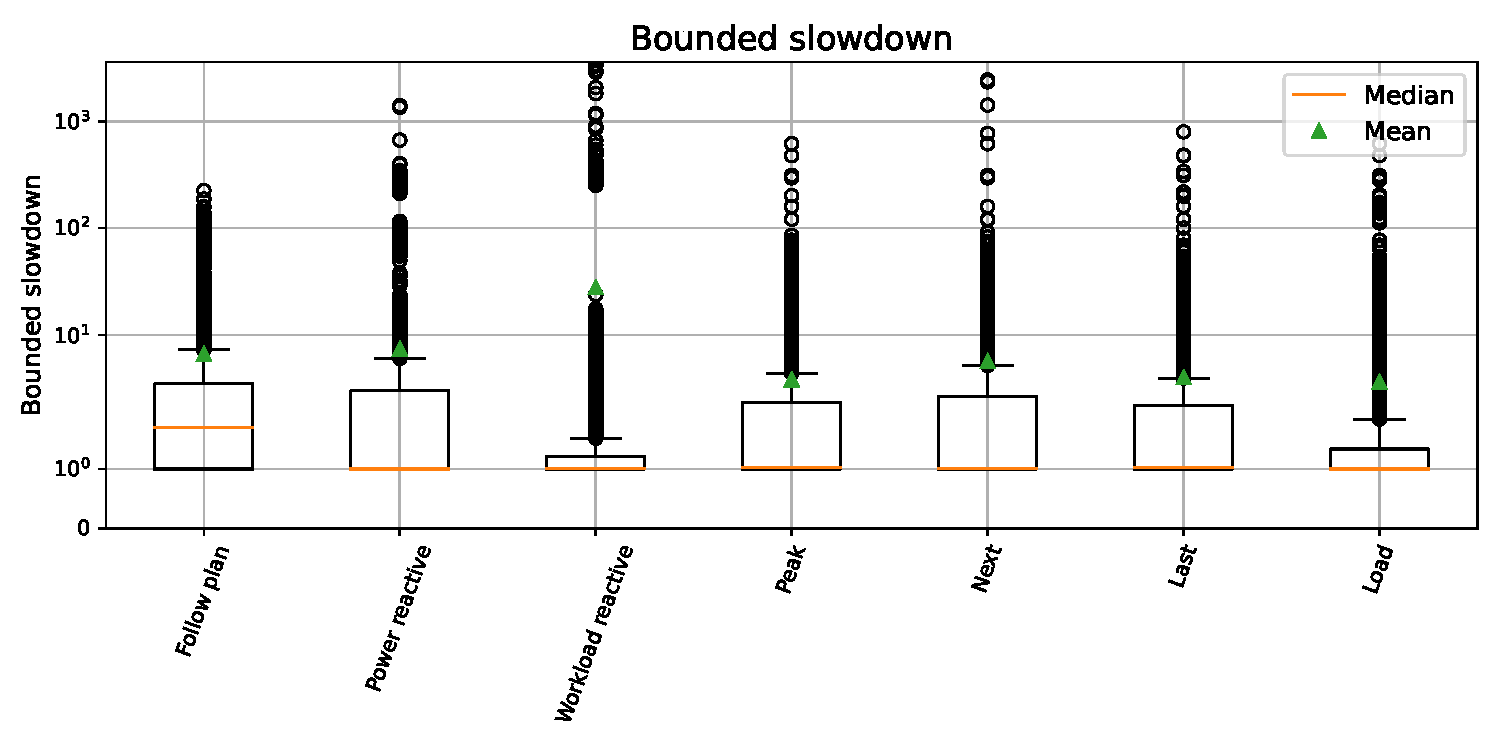
\includegraphics[scale=0.55]{Images/Compensations/slowdown_critical_1.pdf}
    \caption{Bounded slowdown at scenario critical 1.}
    \label{fig:slowdown_critical_1}
\end{figure}

\clearpage

\subsubsection{Scenario Critical 2}

Scenario Critical 2 has more energy (Profile best-case) and the jobs arriving on the third day. The policies do not have a long time to compensate since the load comes on the last day. Figures \ref{fig:SoC_critical_2} and \ref{fig:jobs_critical_2} demonstrate the battery level and finished jobs. 

\begin{figure}[!htb]
    \centering
    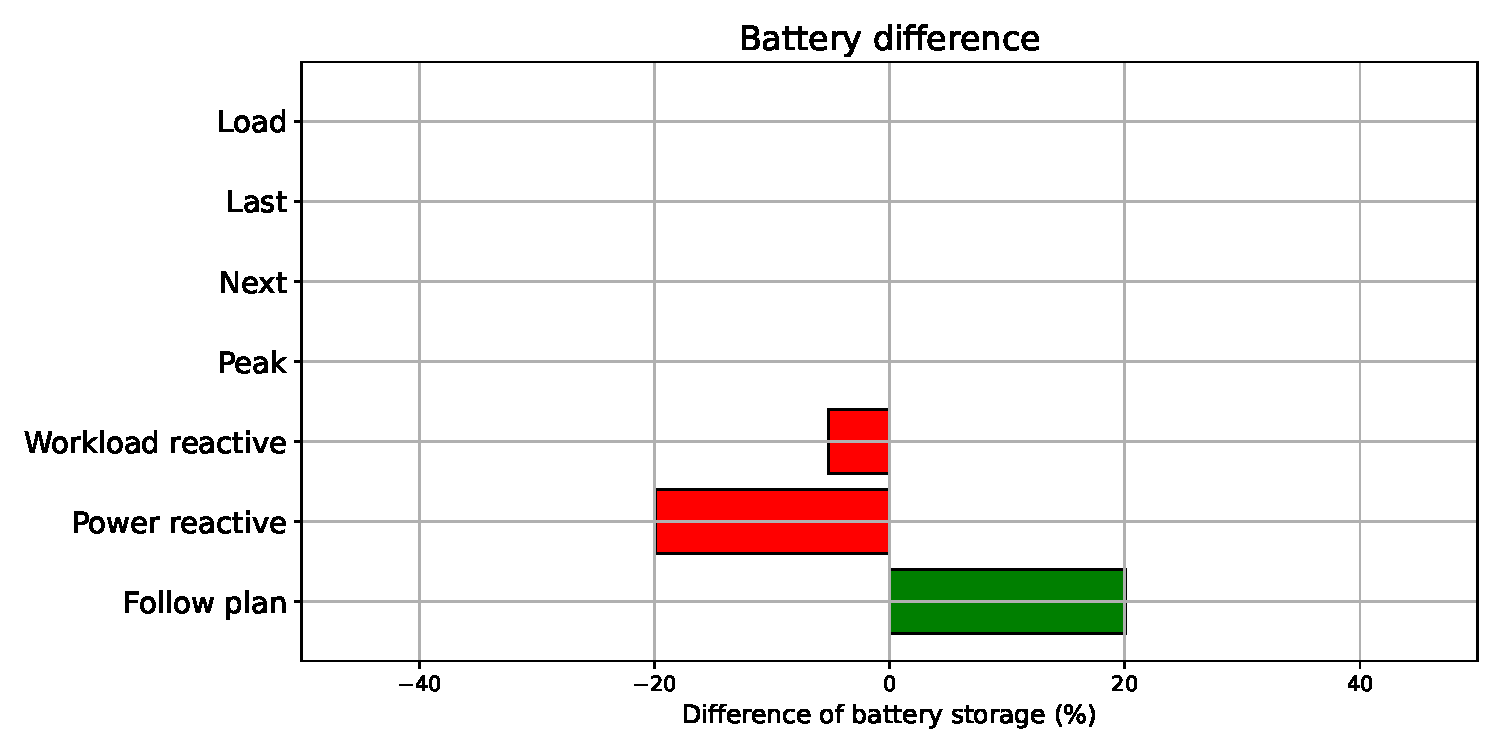
\includegraphics[scale=0.55]{Images/Compensations/battery_critical_2.pdf}
    \caption{Difference between the battery target level (50\%) and the real battery level at the end of the time window for scenario critical 2.}
    \label{fig:SoC_critical_2}
\end{figure}

\begin{figure}[!htb]
    \centering
    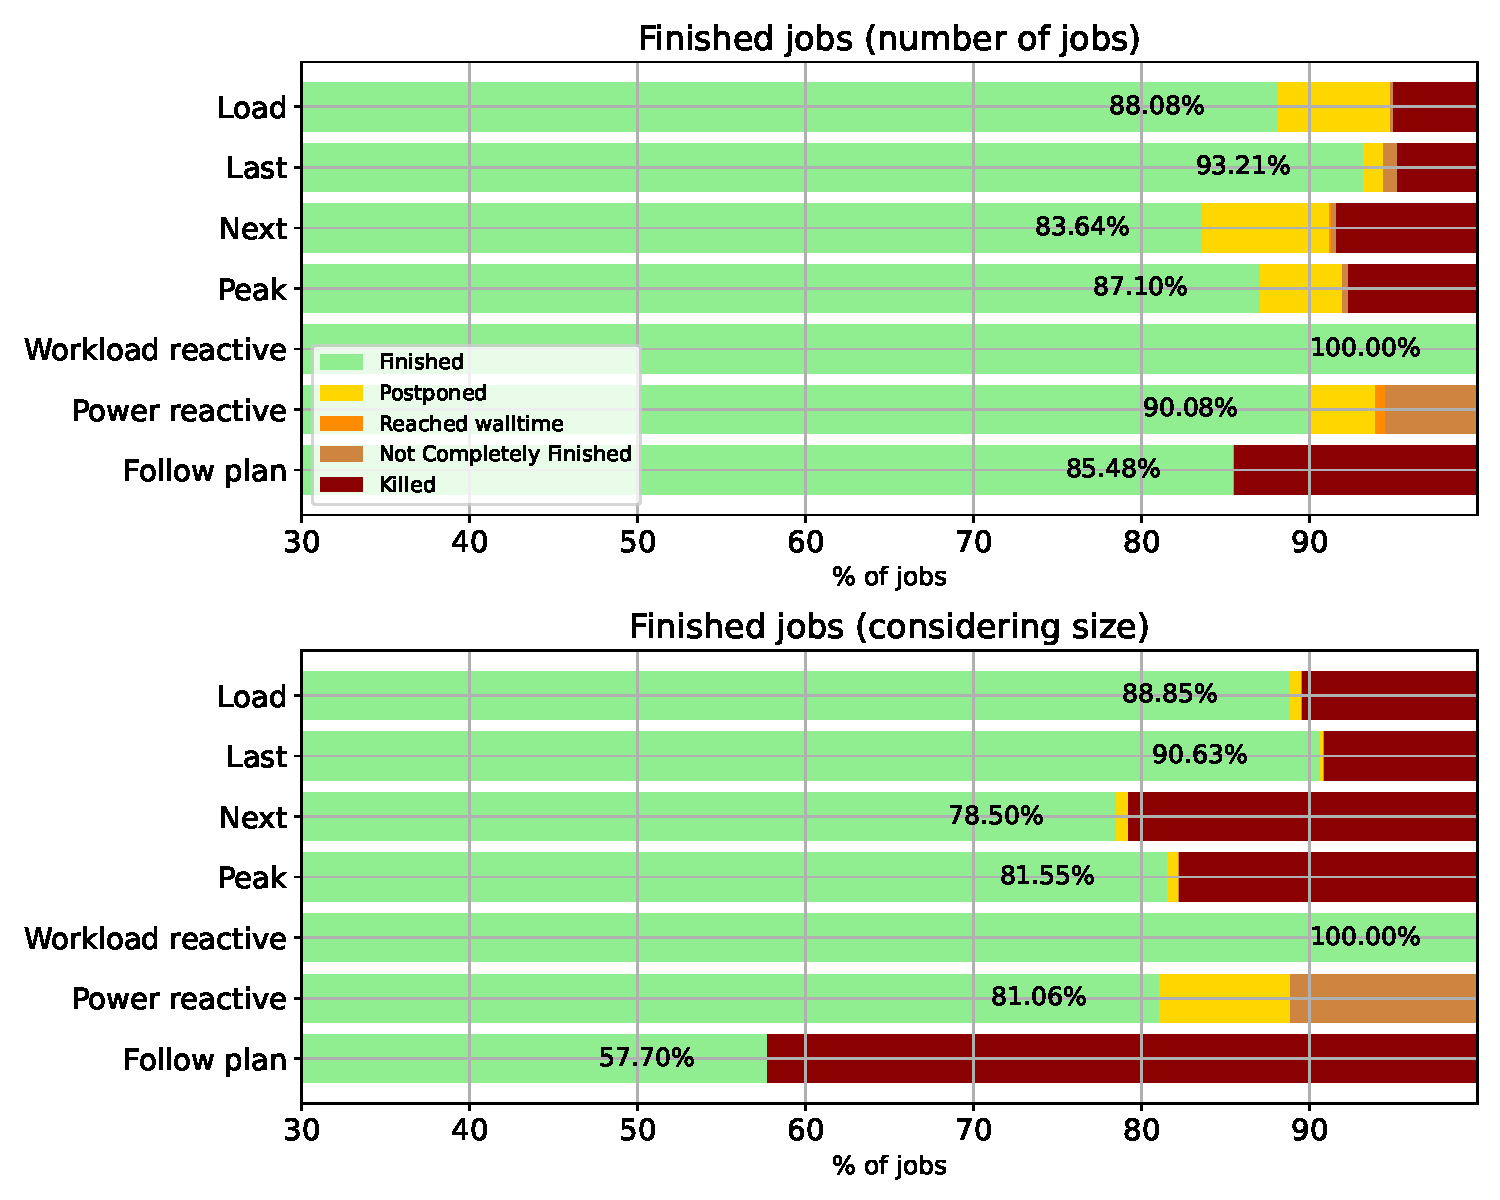
\includegraphics[scale=0.55]{Images/Compensations/jobs_critical_2.pdf}
    \caption{Jobs state at scenario Critical 2. The first graph (above) considers only the number of jobs, ignoring their size. In the second graph (below), the jobs' size is considered.}
    \label{fig:jobs_critical_2}
\end{figure}

\emph{Workload reactive} finished all jobs. This scenario is the best one for this algorithm since it can fulfill the battery in the first two days, consuming all in the last day. Even so, it finishes with a battery deficit (-5.186277\%). \emph{Follow plan} has the second-worst finished jobs and the worst killed jobs (in number) but finishes with a battery surplus of around 20\%. So, it misses the opportunity of using this surplus to avoid killing jobs. Considering the size, it kills more than 40\%. \emph{Power reactive} has the third-best finished jobs (in number), but with a good part not completely finished. These jobs are still running at the end of the time window, so we do not know if they would finish or not. However, it has the third-worst finished jobs considering the size of the jobs. Like in Scenario Critical 1, \emph{Power reactive} has a large battery deficit, with around -20\%. All policies have a perfect battery level, finishing with the SoC at around 50\% (the target level). All policies kill fewer jobs than the \emph{Follow plan}, using the higher production to do so. However, they kill jobs to arrive at the battery target level, avoiding using more battery than predicted.

Just \emph{Next} policy finishes fewer jobs than \emph{Follow plan} in number, but more considering the size. This policy consumes all incoming energy as soon as possible, not having too much to use on the last day. \emph{Peak} has the third-worst finished jobs metric considering the number, worst than \emph{Power reactive}. This policy puts the surplus energy in the moment with less energy (negative peak). This behavior creates a more constant number of servers available during the time window. However, this case has a load in the end. So, reintroducing the energy in the \emph{Peak} approach does not help to finish more jobs. On the other hand, \emph{Peak} finishes bigger jobs than \emph{Power reactive}. It can finish bigger jobs due to its constant number of servers behavior. However, since the majority of jobs arrive at the end, it is better to place the positive compensations at the end (like \emph{Load} and \emph{Last}).

We can see a small difference in jobs finished (in number) between \emph{Peak} and \emph{Load}, where \emph{Load} puts the energy in the moments with a higher difference between demand and production. It helps to increase almost 1\% of finished jobs and decreases around 2\% of killed jobs. Besides, \emph{Load} can increase the number of bigger jobs finished compared to the \emph{Peak} policy. Nevertheless, the best results come from \emph{Last}. This policy stocks all surplus at the last moment, allowing to execute more jobs. It can finish 3.13\% (number of jobs) more than the third-best, the only above 90\% finished jobs considering the size (besides \emph{Workload reactive}), and having a perfect level of battery at the end of the time window.

Considering the wasted energy, Figure \ref{fig:energy_critical_2} illustrates the results in this scenario. Again, \emph{Workload reactive} has the lowest wasted energy due to its workload reactiveness approach. The worst one is \emph{Power reactive}, for the same reason as scenario Critical 1. It turns on and increases the speed according to the incoming power, not the demand. \emph{Follow plan} has not-so-bad wasted energy, even with a high killed jobs. \emph{Peak} and \emph{Next} wasted more than the \emph{Follow plan}. Both policies place the energy at the wrong moments. For example, if \emph{Next} has a positive compensation (increase the usage) in step 1, it will increase in step 2. However, the demand is in the end. Then, the energy is wasted on idle servers. \emph{Peak} policy has a similar problem. With the load in the beginning, it was not a problem for \emph{Peak} (it can delay the jobs for later execution). Nevertheless, in this scenario, it puts positive compensations in the moments with lower usage, leading to more moments with idle servers. On the other hand, \emph{Last} and \emph{Load} have better energy usage than the \emph{Follow plan}. Both policies put the energy in the right moment (last steps).

\begin{figure}[!htb]
    \centering
    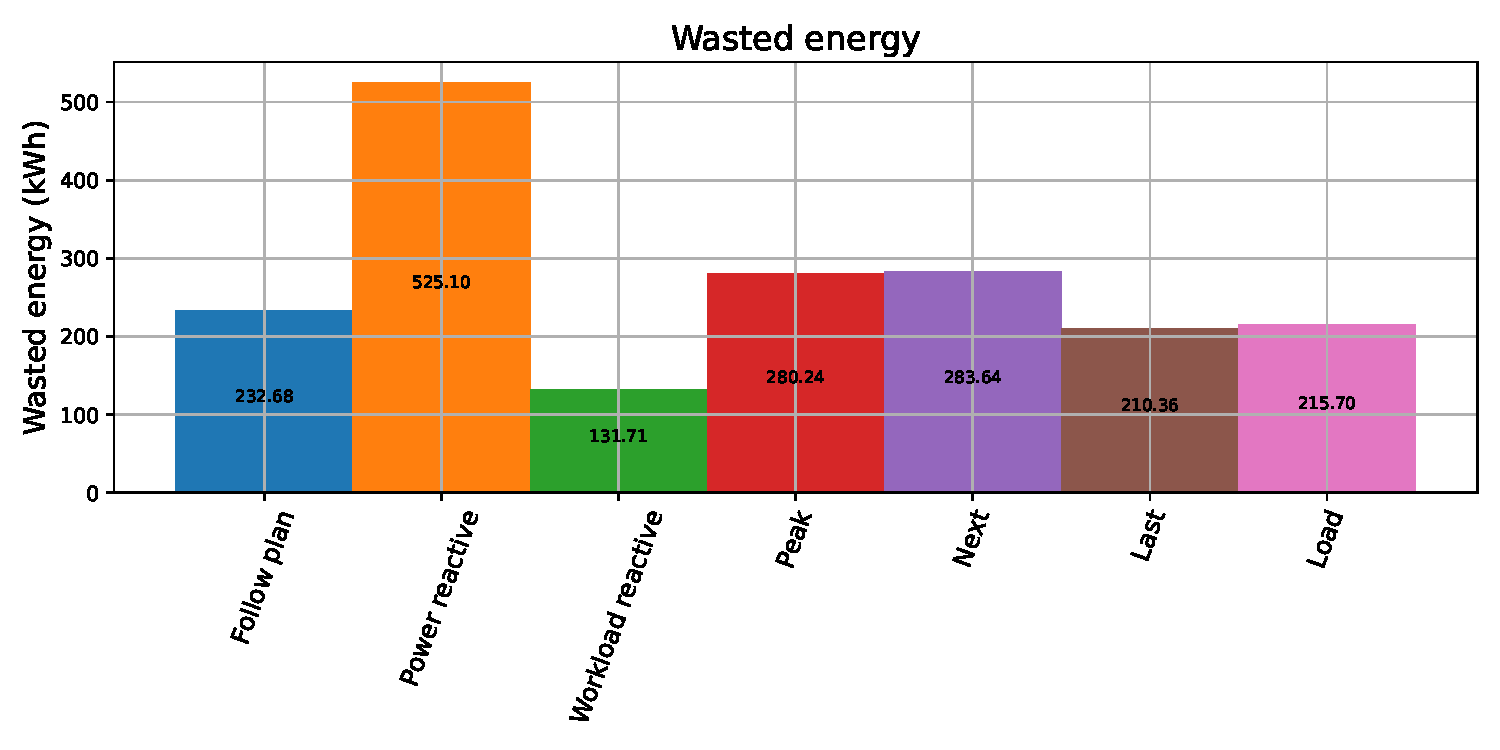
\includegraphics[scale=0.55]{Images/Compensations/energy_critical_2.pdf}
    \caption{Wasted energy at scenario Critical 2.}
    \label{fig:energy_critical_2}
\end{figure}

Regarding the bounded slowdown, Figure \ref{fig:slowdown_critical_2} shows the results. \emph{Workload reactive} has the best results due to its workload reactiveness. Without the SoC problem from the previous scenario, it can execute all jobs as soon as they arrive. The policies present a better median than \emph{Follow plan} but a higher mean, due to several jobs with bounded slowdown higher than 100. Yet, since \emph{Last}, \emph{Peak}, and \emph{Load} finish more jobs than \emph{Follow plan}, it is complicated to compare them.

\begin{figure}[!htb]
    \centering
    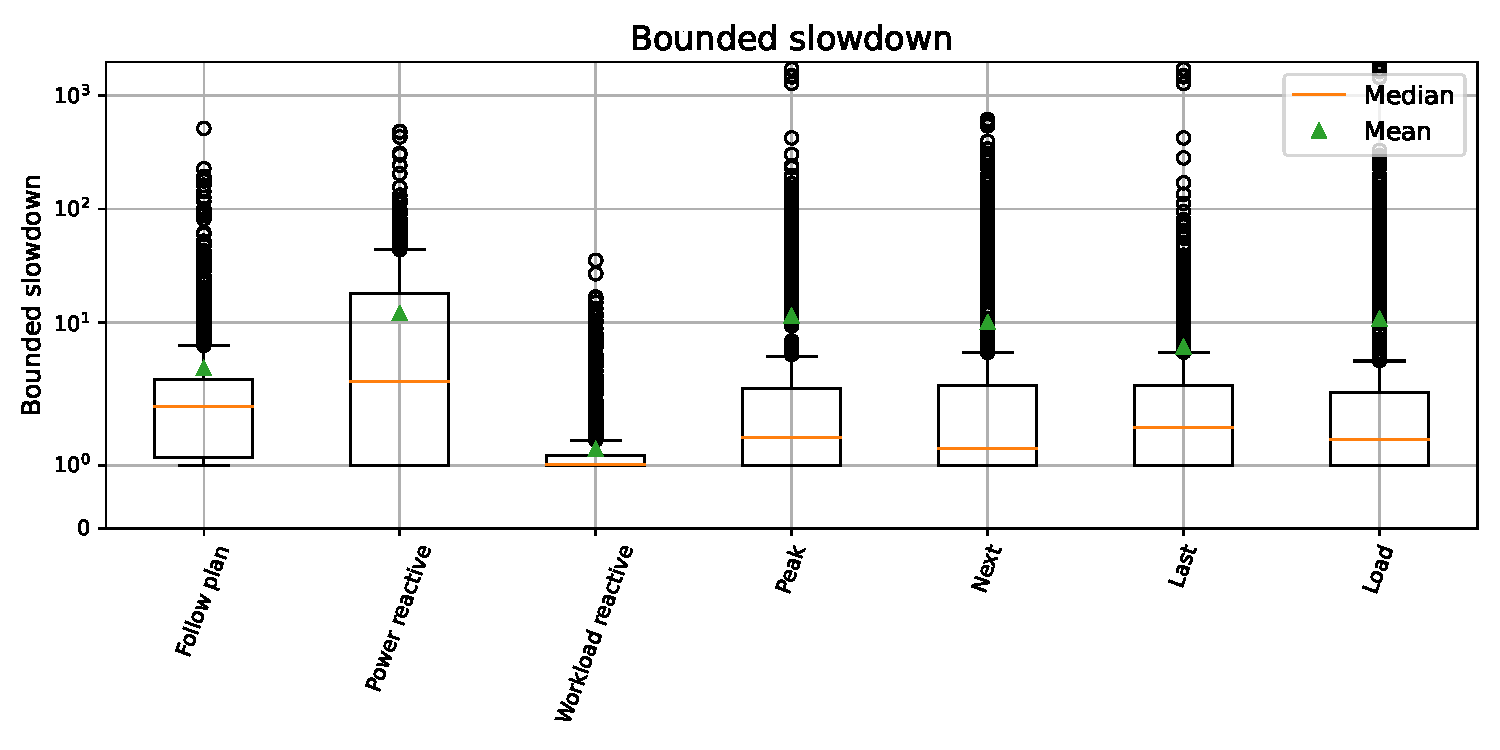
\includegraphics[scale=0.55]{Images/Compensations/slowdown_critical_2.pdf}
    \caption{Bounded slowdown at scenario Critical 2.}
    \label{fig:slowdown_critical_2}
\end{figure}

\clearpage

\subsubsection{Scenario Critical 3}
Scenario 3 introduces less energy than predicted with the jobs arriving on the first day. Figure \ref{fig:SoC_critical_3} gives the final battery level in this scenario. This figure demonstrates that the policies finished closer to the target level than the baselines, with -6.177244\% in the worst case (\emph{Load}). This scenario is particularly difficult to finish at 50\% since the policies migrate power to the first day expecting to compensate for it on the second and third days. However, it receives less energy than expected, being a little far from the target level. Nevertheless, the policies are way better compared to the \emph{Workload reactive}, \emph{Power reactive}, and \emph{Follow plan}.

\begin{figure}[!htb]
    \centering
    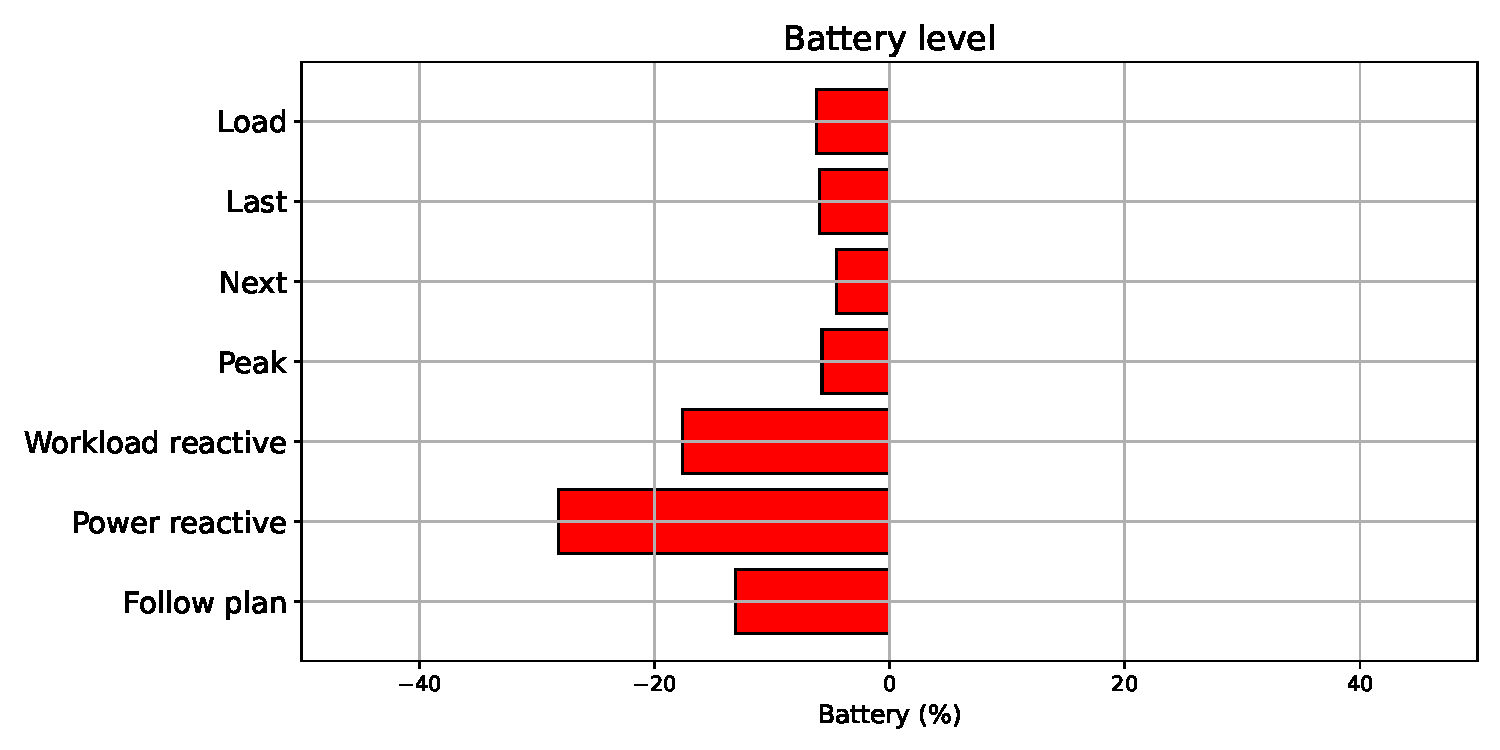
\includegraphics[scale=0.55]{Images/Compensations/battery_critical_3.pdf}
    \caption{Difference between the battery target level (50\%) and the real battery level at the end of the time window for scenario critical 3.}
    \label{fig:SoC_critical_3}
\end{figure}

Concerning finished jobs, Figure \ref{fig:jobs_critical_3} illustrates the results. As presented in scenario 1, \emph{Workload reactive} has a problem with the load on the first day because it will place all jobs as soon as they arrive, drying the battery. We can see that scenario 3 is even worst, having more than 20\% killed jobs in number and more than 40\% in size. \emph{Power reactive} finishes more jobs than any other algorithm, with 85.60\% (in number) and 61.43\% (in size). This algorithm follows the real production to set the servers' speeds. This behavior helps to start several jobs, but it can not maintain the jobs running when the battery arrives at $SoC_{min}$. So, it has more than 10\% of killed jobs considering the number and almost 40\% considering the size. \emph{Follow plan} finishes more jobs than the policies in both number and size. However, it kills several jobs, with more than 20\% in number and almost 50\% in size (the worst result). 

\begin{figure}[!htb]
    \centering
    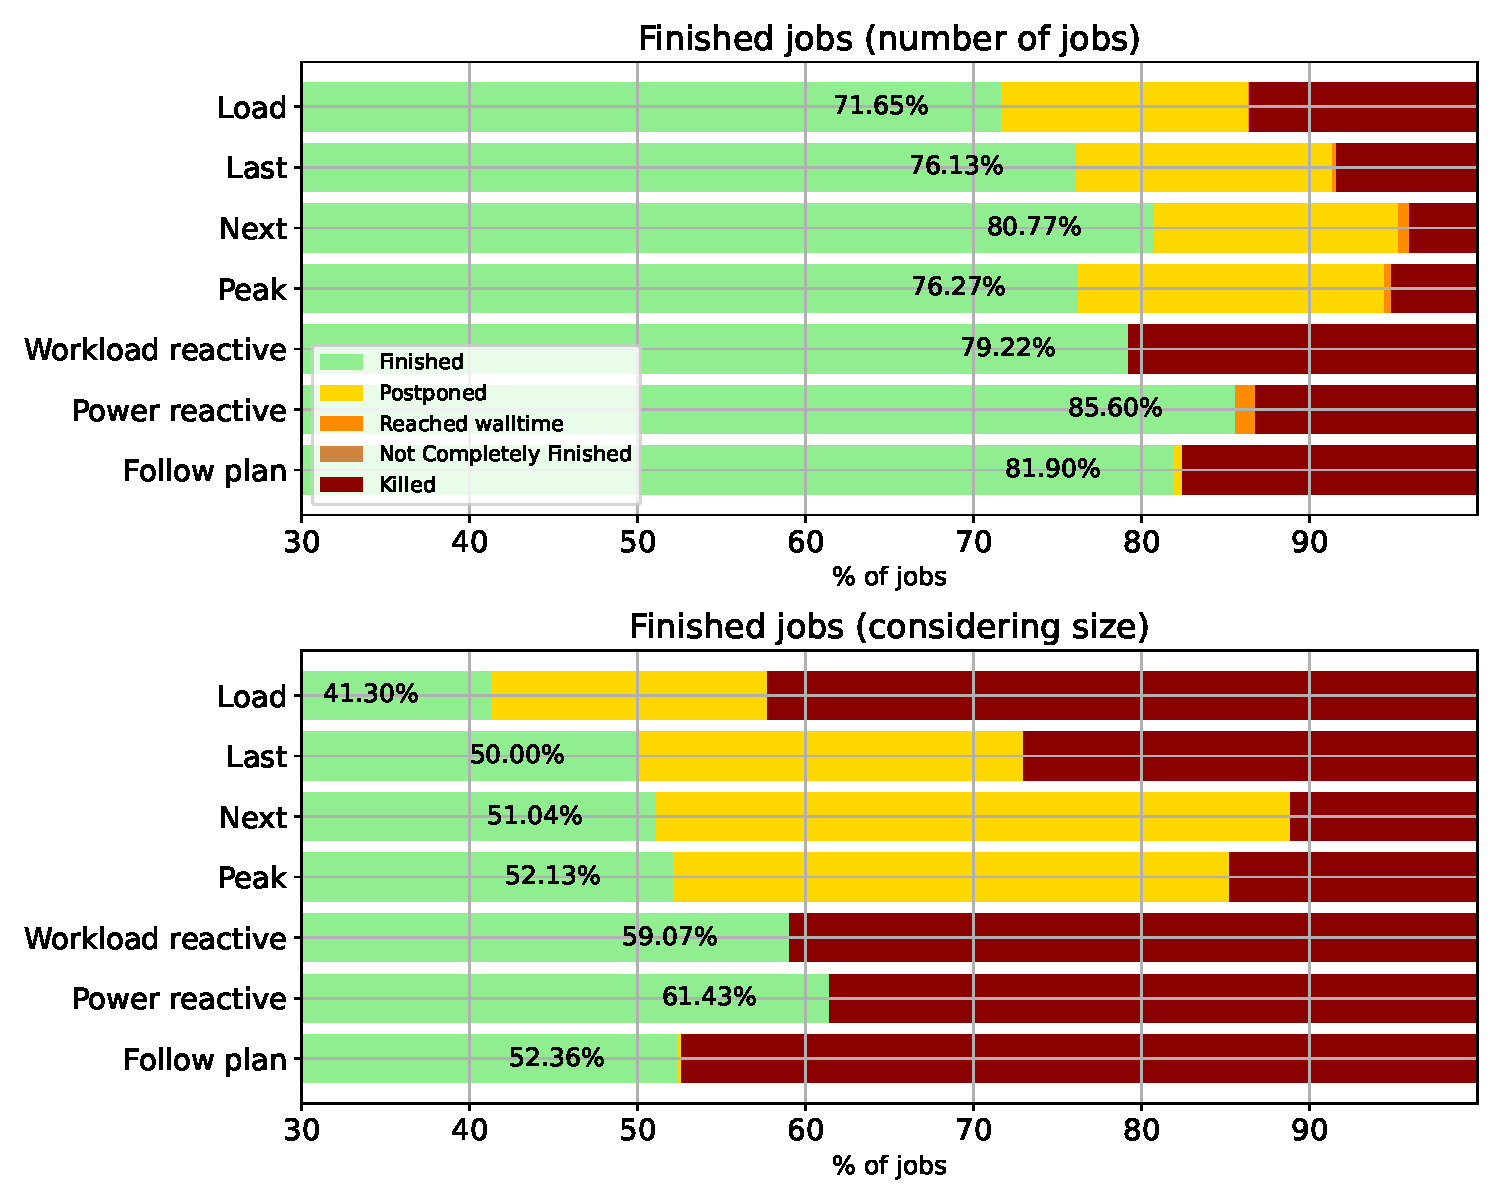
\includegraphics[scale=0.55]{Images/Compensations/jobs_critical_3.pdf}
    \caption{Jobs state at scenario critical 3. The first graph (above) considers only the number of jobs, ignoring their size. In the second graph (below), the jobs' size is considered.}
    \label{fig:jobs_critical_3}
\end{figure}

Among the policies, \emph{Load} has the worst result of finished and killed jobs in both number and size, compared to the other policies. In this scenario, \emph{Load} puts any positive compensation on the first day, approximating too fast to $SoC_{min}$. Then, it has to kill several jobs to avoid this boundary. This result shows that \emph{Load} aggressivity does not always worth it. On the other hand, \emph{Next} stays close to the SoC planned. In this case, it can manage the SoC better, finishing more than 80\% of jobs in number. Among the policies, \emph{Next} is only worst than \emph{Peak}. As mentioned before, \emph{Peak} can smooth the peaks maintaining more servers available constantly. We can see that it finishes fewer jobs in number than \emph{Next} but more in size. \emph{Peak} has a similar result to \emph{Follow plan}, using less battery and killing fewer jobs, highlighting the need for reactivity.

Figure \ref{fig:energy_critical_3} shows the wasted energy in this scenario. We can see that all policies present lower wasted energy than the baselines, a crucial result in a scenario with less energy available. \emph{Next} policy wasted 45.96\% less energy than \emph{Workload reactive} (the best baseline). \emph{Load} has the worst wasted energy among the policies due to the number of killed jobs. Even so, \emph{Power reactive} has lower killed jobs than \emph{Load}, but it has higher wasted energy. \emph{Power reactive} follows the power available, turning on servers according to the power available. Therefore, it expends more energy than the other algorithms in transition states.

\begin{figure}[!htb]
    \centering
    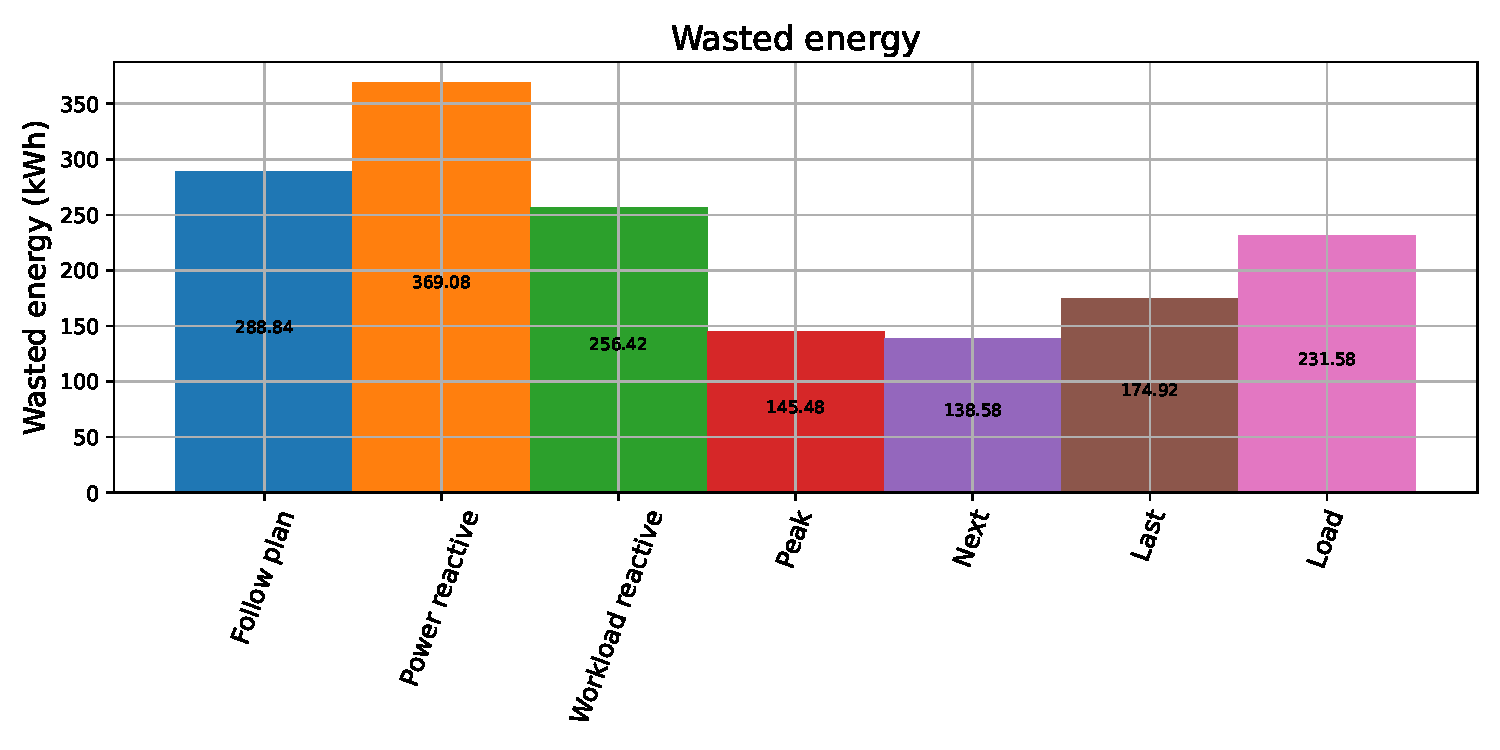
\includegraphics[scale=0.55]{Images/Compensations/energy_critical_3.pdf}
    \caption{Wasted energy at scenario critical 3.}
    \label{fig:energy_critical_3}
\end{figure}

Finally, Figure \ref{fig:slowdown_critical_3} shows the bounded slowdown. \emph{Workload reactive} has a similar result to Scenario 1. When it arrives at $SoC_{min}$, it has a long time without servers available, increasing the waiting time and slowdown for some jobs. However, it still has a very low median, showing that the majority has a small slowdown. In this scenario, the policies let the jobs wait longer, delaying the starting time for the moment with enough energy to finish them. So, the policies have higher mean and median slowdowns. 

\begin{figure}[!htb]
    \centering
    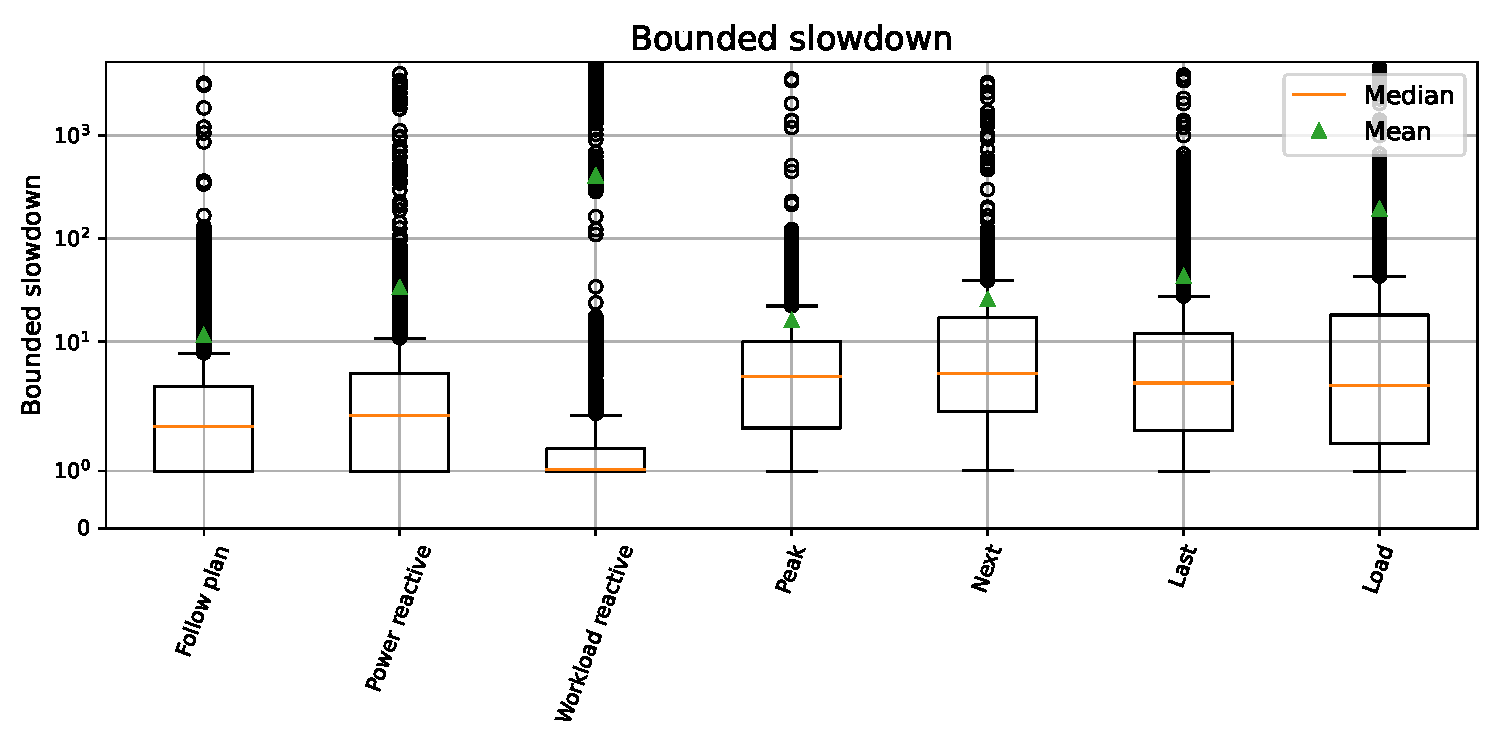
\includegraphics[scale=0.55]{Images/Compensations/slowdown_critical_3.pdf}
    \caption{Bounded slowdown at scenario critical 3.}
    \label{fig:slowdown_critical_3}
\end{figure}

\clearpage

\subsubsection{Scenario Critical 4}

The last critical scenario is the harder one, with less energy and jobs arriving on the last day. Figure \ref{fig:SoC_critical_4} shows the impact on the battery level. Both \emph{Workload reactive} and \emph{Power reactive} finished with a deficit higher than 30\%, with 31.45\% and 30.78\%. Both ended the battery with less than the $SoC_{min}$ of 20\% (18.55\% and 19.22\%). \emph{Follow plan} finished with the SoC at 35.72\% (-14.28\%), far from the target level. Nevertheless, the policies finished very close to 50\%. Since the first two days provide less energy, the policies can adapt the usage of the last day to approximate the target level. However, Figure \ref{fig:jobs_critical_4} shows the impact on QoS.

\begin{figure}[!htb]
    \centering
    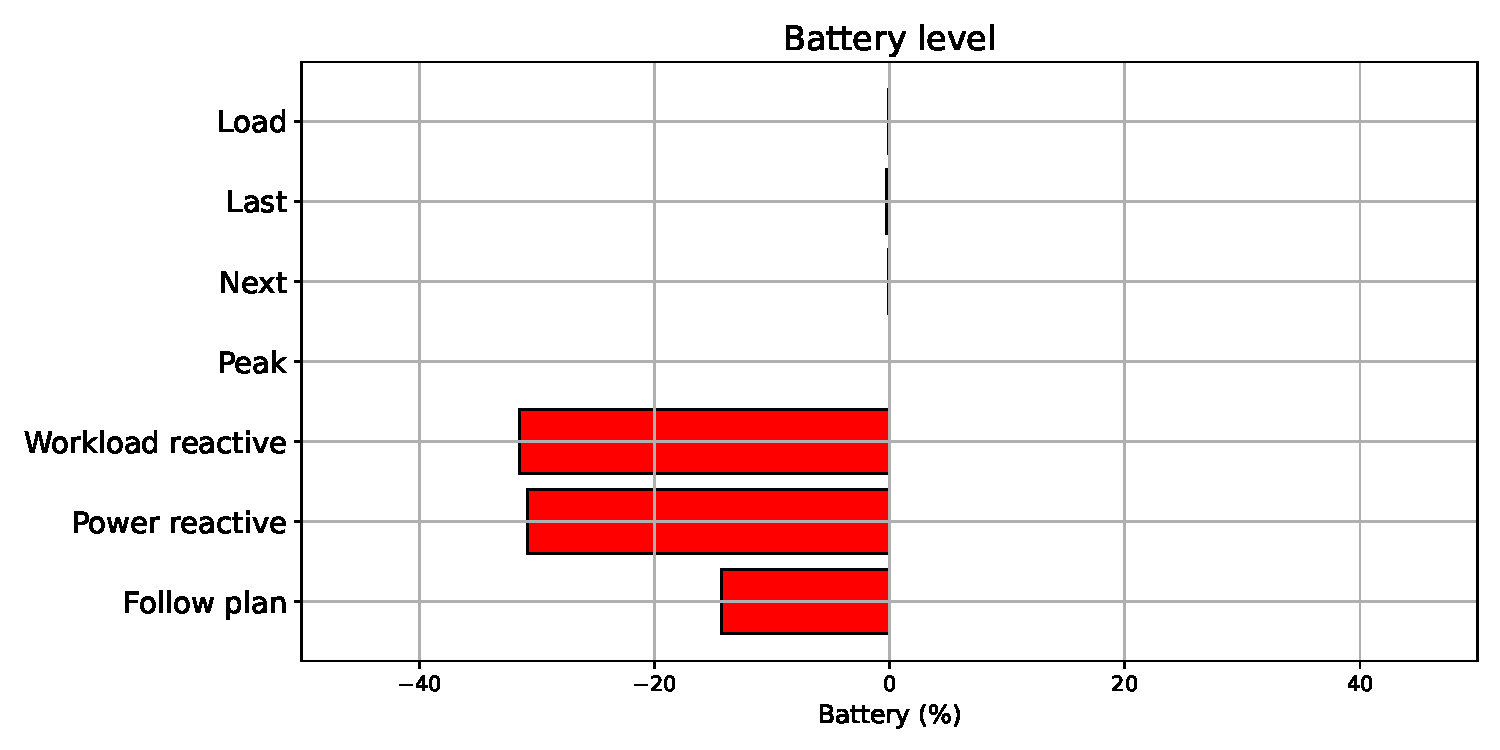
\includegraphics[scale=0.55]{Images/Compensations/battery_critical_4.pdf}
    \caption{Difference between the battery target level (50\%) and the real battery level at the end of the time window for scenario critical 4.}
    \label{fig:SoC_critical_4}
\end{figure}

\begin{figure}[!htb]
    \centering
    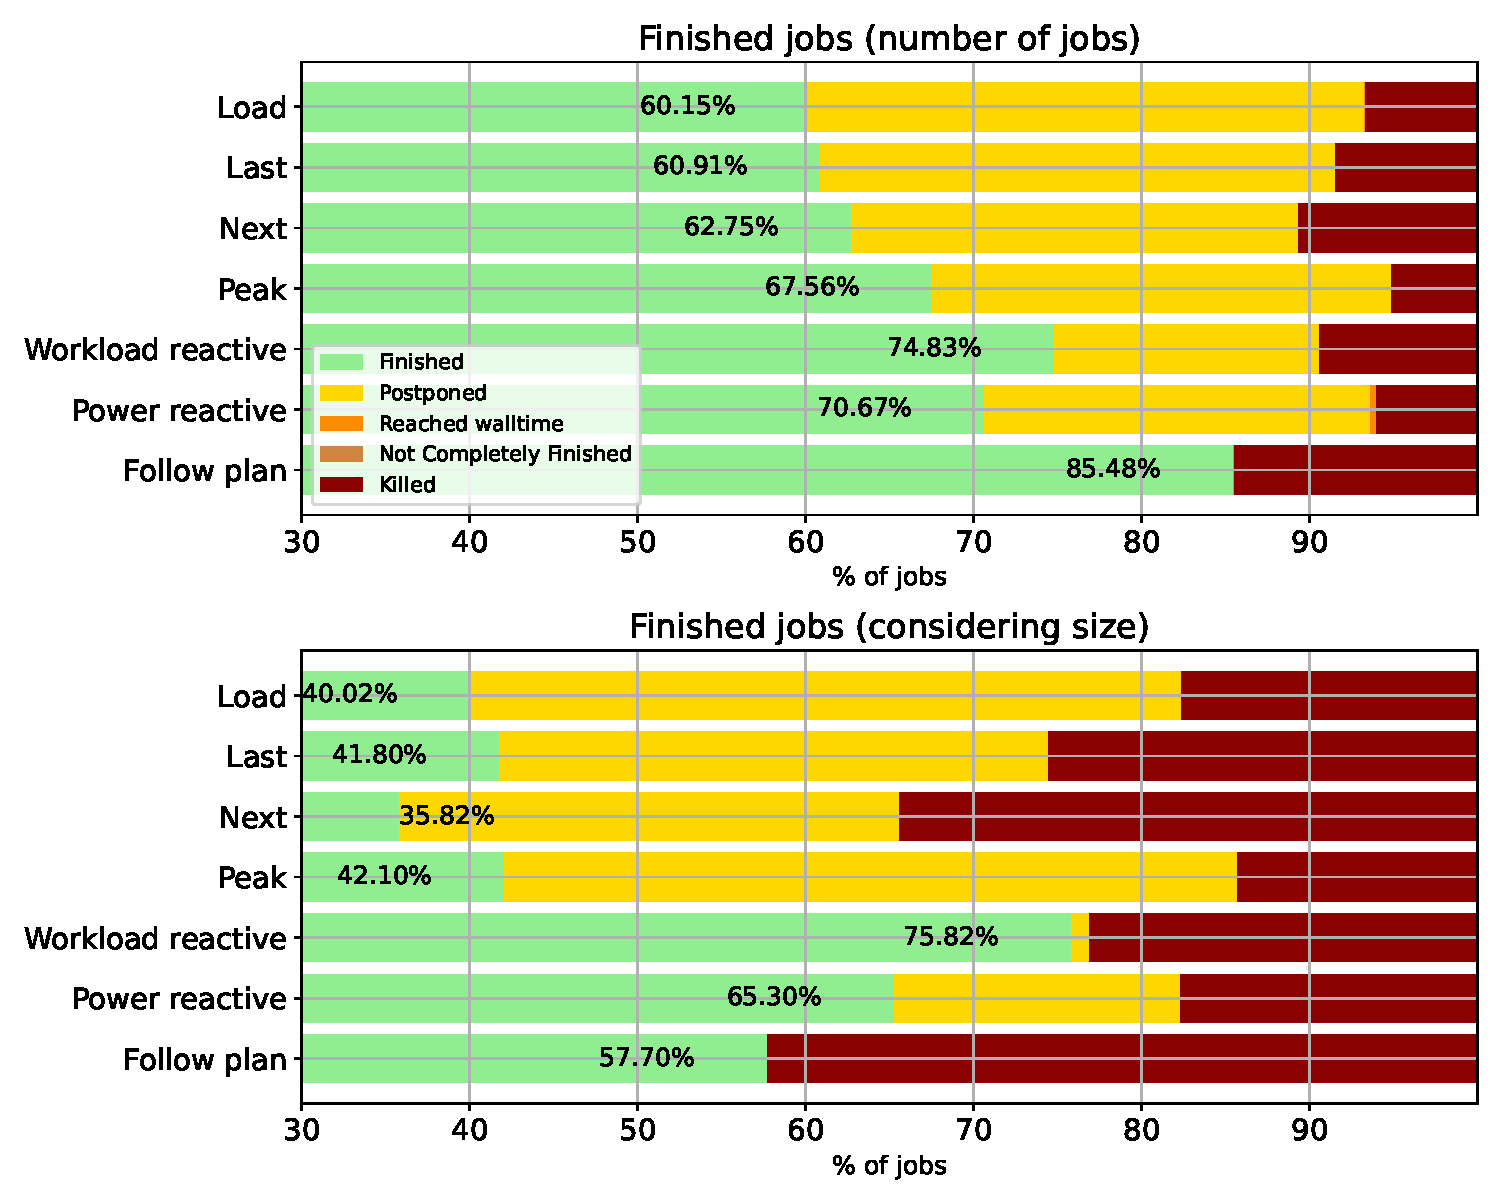
\includegraphics[scale=0.55]{Images/Compensations/jobs_critical_4.pdf}
    \caption{Jobs state at scenario critical 4. The first graph (above) considers only the number of jobs, ignoring their size. In the second graph (below), the jobs' size is considered.}
    \label{fig:jobs_critical_4}
\end{figure}

Figure \ref{fig:jobs_critical_4} demonstrates that the policies finished fewer jobs than the baselines in number and size. Considering the number of killed jobs, only \emph{Peak} kills fewer jobs than the other algorithms, but very close to the \emph{Power reactive}. In a scenario with less energy, the policies will impact the QoS, approximating the battery's SoC to the target level. \emph{Follow plan} has the best number of finished jobs, but it finishes mainly small jobs. It kills more than 40\% of the jobs considering the size (the worst result). \emph{Workload reactive} has the second-best finished jobs in number and the best in size. However, \emph{Workload reactive} kills more jobs in number than \emph{Power reactive}, \emph{Peak}, \emph{Last}, and \emph{Load}. The battery goes below 20\% on the last day, killing several jobs. The same happens to \emph{Power reactive}. Even with several jobs killed, Figure \ref{fig:energy_critical_4} indicates that all policies wasted less energy than the baselines. The policies adapt the plan to maximize energy usage. In a scenario with low energy production, it is essential to improve energy usage. Figure \ref{fig:slowdown_critical_4} shows that the policies also impact the Slowdown, having worst results than the baselines. 

\begin{figure}[!htb]
    \centering
    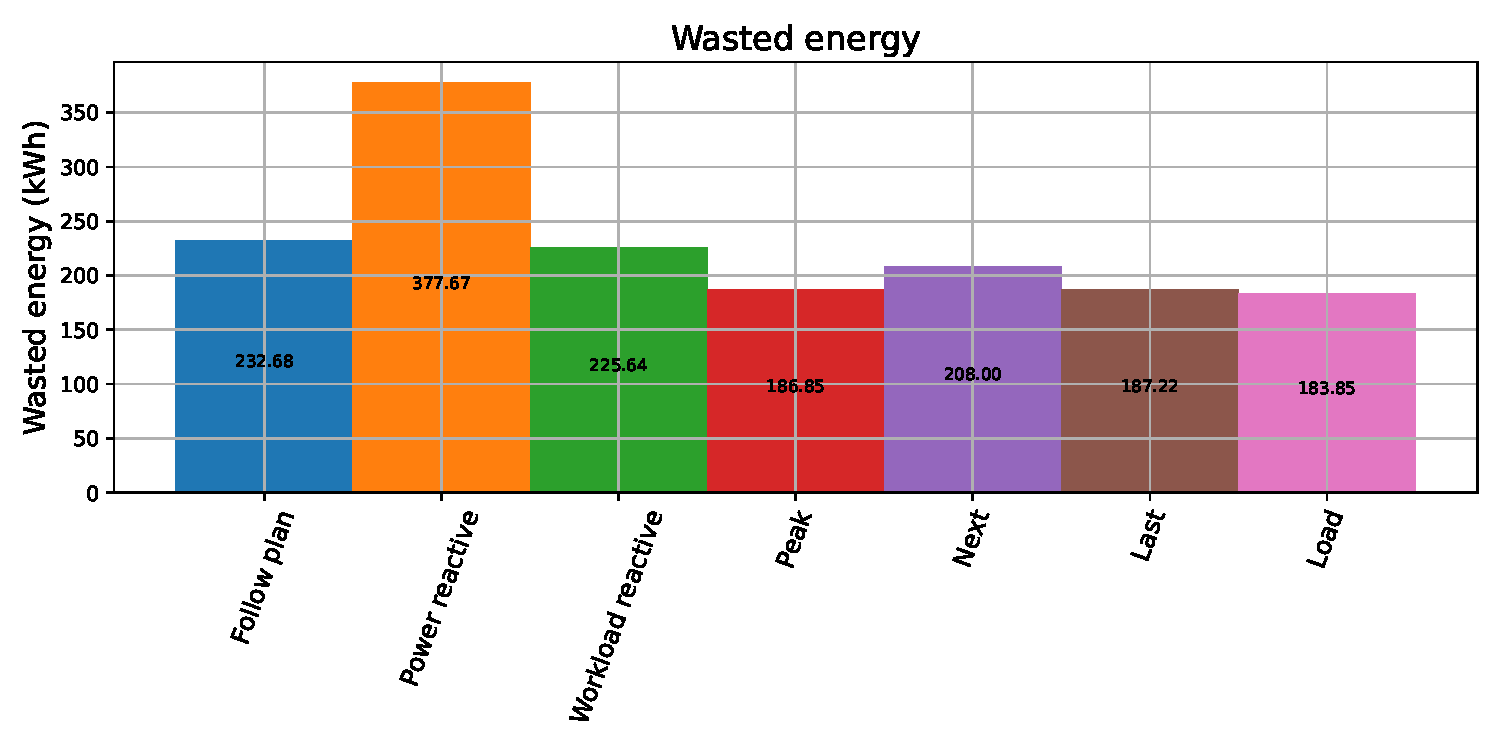
\includegraphics[scale=0.55]{Images/Compensations/energy_critical_4.pdf}
    \caption{Wasted energy at scenario critical 4.}
    \label{fig:energy_critical_4}
\end{figure}

\begin{figure}[!htb]
    \centering
    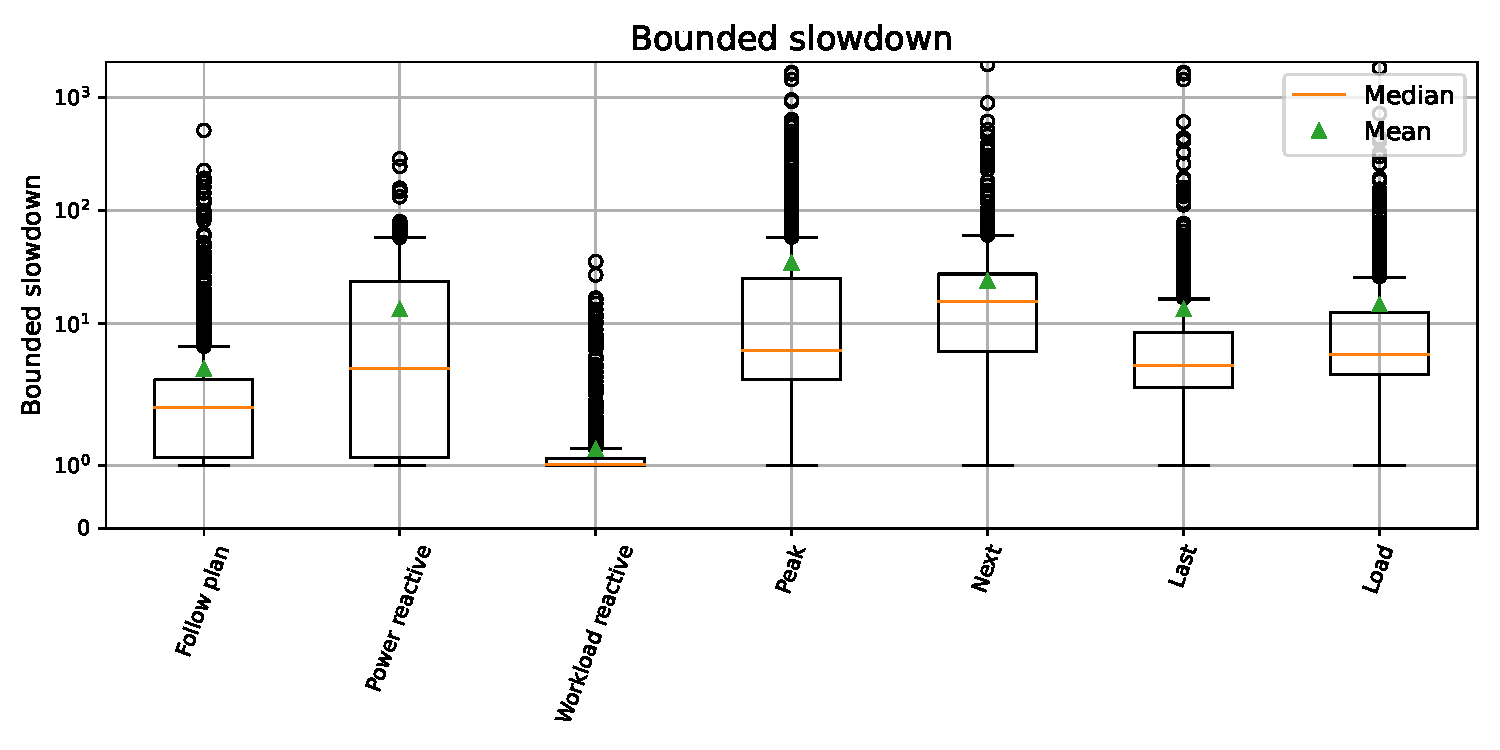
\includegraphics[scale=0.55]{Images/Compensations/slowdown_critical_4.pdf}
    \caption{Bounded slowdown at scenario critical 4.}
    \label{fig:slowdown_critical_4}
\end{figure}

The results in this scenario indicate that the policies degrade the QoS (finished jobs and slowdown) to approximate the target level. The policies' compensation imposes the adaptations on power usage and server configuration. In this scenario, these adaptations demand an available servers reduction or reduce their speed. 

\clearpage

\subsection{Random cases}

After presenting the critical scenarios, this section demonstrates the results of 100 random cases. These random cases vary the power production and workload randomly, following a Gaussian noise. So, they are not always the worst or best, like in critical scenarios. We do not present the slowdown in this scenario. The workload and power productions vary a lot between executions. So, it is inappropriate to compare them. First, Figure \ref{fig:SoC_diff} illustrates the state of charge difference from the target level. The red line indicates the perfect SoC at the end of the time window (0\% of difference from the target level). We can see that the three baselines (\emph{Workload reactive}, \emph{Power reactive}, and \emph{Follow plan}) have a large variance in the results. An important thing to notice is that even in non-critical scenarios, the minimal values of \emph{Workload reactive} and \emph{Power reactive} can arrive at -30\%. This value means they finished with the battery level at 20\%, which is the $SoC_{min}$. \emph{Follow plan} finishes with a higher Median and Mean, indicating that it saves more energy than the other algorithms. However, it also has a large variance.

\begin{figure}[!htb]
    \centering
    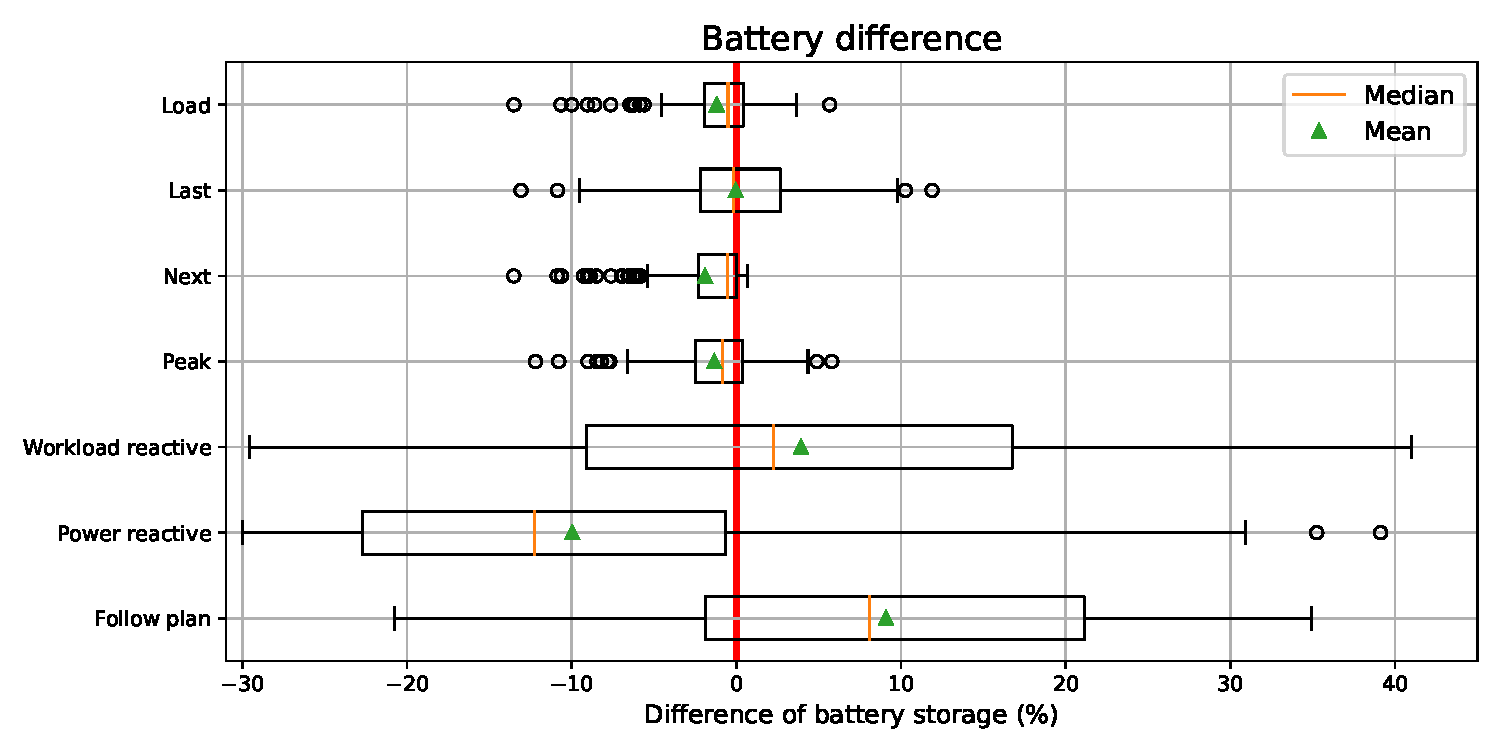
\includegraphics[scale=0.55]{Images/Compensations/battery_diff.pdf}
    \caption{Difference between the battery target level (50\%) and the real battery level at the end of the time window at 100 random cases. The line shows the standard deviation.}
    \label{fig:SoC_diff}
\end{figure}

The policies maintain the SoC between -10\% and 10\%, with some outliers below/above these values. The median and mean are very close to the target level, showing they can approximate the target level which is their main objective. \emph{Last} has the larger variance among the policies, but with median and mean almost perfect. This heuristic compensates in the last moments. Sometimes, this behavior can reduce the possibility to use the energy since the heuristic will not have enough time. 

Regarding the QoS, Figures \ref{fig:finished_diff} and \ref{fig:killed_diff} illustrate the finished and killed jobs. \emph{Workload reactive} has the best percentage of finished jobs (in number and size). This result is expected since this algorithm dries the battery to maximize the number of finished jobs. \emph{Workload reactive} also has low median and mean killed jobs. However, concerning the number of killed jobs, it has some results higher than 15\% (with two higher than 20\%). \emph{Power reactive} has good finished jobs but never finishes more than 97.90\%. This algorithm also has some executions with more than 15\% of killed jobs in number. The worst execution is \emph{Follow plan}, with high mean and median killed jobs (in number and size) and low finished jobs in size. Combining the state of charge from Figure \ref{fig:SoC_diff} with this result, we can notice that \emph{Follow plan} misses opportunities of using more power to execute more jobs or maintain big jobs running.

\begin{figure}[!htb]
    \centering
    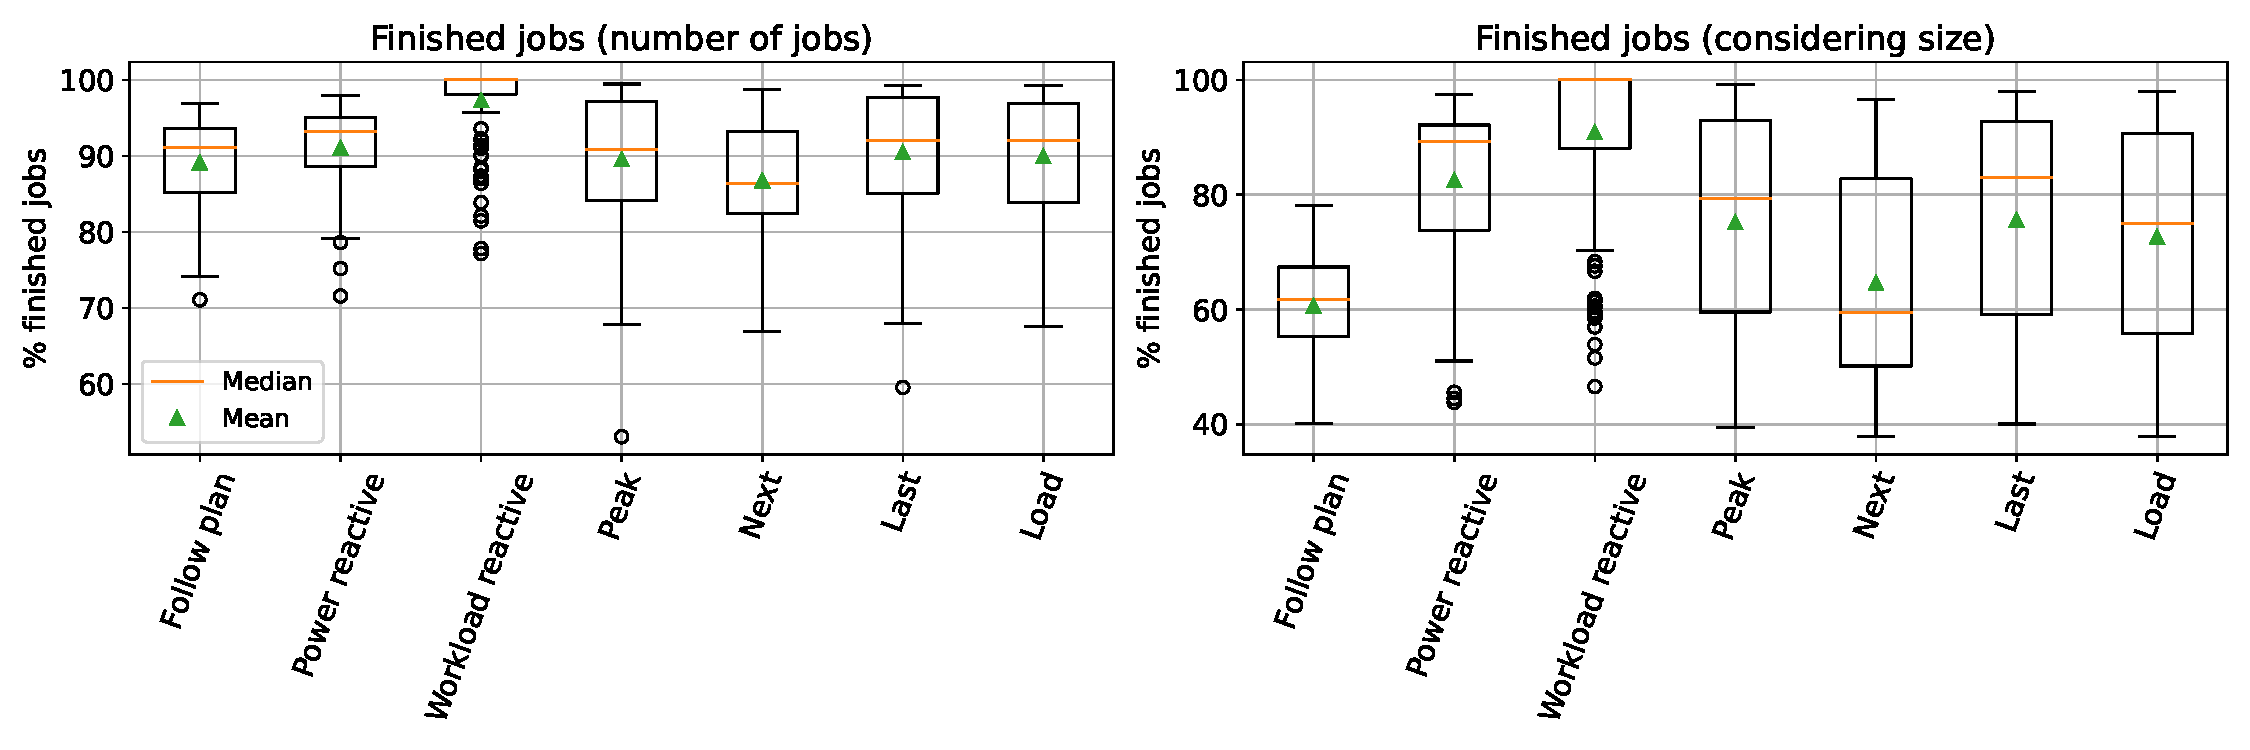
\includegraphics[scale=0.38]{Images/Compensations/finished_diff.pdf}
    \caption{Finished jobs at 100 random cases.}
    \label{fig:finished_diff}
\end{figure}

\begin{figure}[!htb]
    \centering
    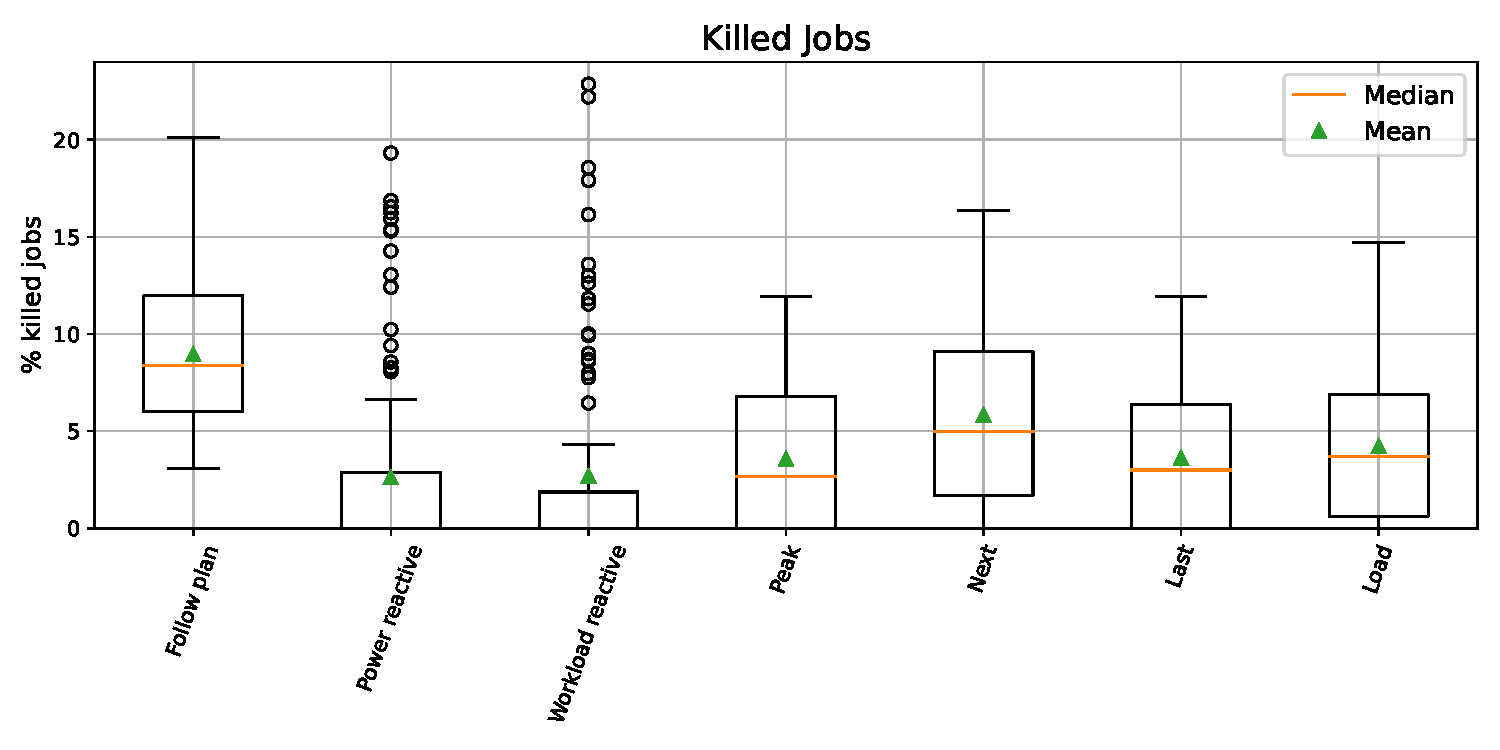
\includegraphics[scale=0.38]{Images/Compensations/killed_diff.pdf}
    \caption{Killed jobs at 100 random cases.}
    \label{fig:killed_diff}
\end{figure}

The policies have good finished jobs (in number), with \emph{Last} being a little below the \emph{Power reactive}. They also have some executions with almost 100\% of finished jobs (above 99\%). Considering the number of jobs killed, \emph{Last} and \emph{Peak} maintain the results in control, with no value above 15\%. \emph{Load} has the worst case close to 15\% and \emph{Next} with 16.37\%. Considering the size, the policies have worst results than \emph{Power reactive} and \emph{Workload reactive}. These jobs are harder to maintain running because they demand more time and power. So, the policies can kill them to guarantee the battery target level.

Finally, Figure \ref{fig:energy_diff} illustrates the wasted energy of over 100 executions. The best execution is \emph{Workload reactive}. As mentioned before, this heuristic focus on running jobs, letting the servers down until they are needed. Besides, the DPM technique reduces wasted energy. The worst algorithm is \emph{Power reactive}. This algorithm turns on servers even if they are not necessary. \emph{Follow plan} is better than three policies (\emph{Peak}, \emph{Next}, and \emph{Load}). The best policy is \emph{Last}, mainly because it runs more jobs than the other policies and \emph{Follow plan}. While \emph{Follow plan} uses only the energy planned, the policies can reintroduce the energy from power variations. However, these policies change the usage using simplified heuristics. So, they can place the energy in moments without jobs to run. \emph{Last} is the policy that suffers the least from this problem because it places the compensations in the end. Therefore, it can re-migrate this energy at any moment before the end. Section \ref{sec:compensation_discussion} presents an overview of the advantages and problems of these policies. 

\begin{figure}[!htb]
    \centering
    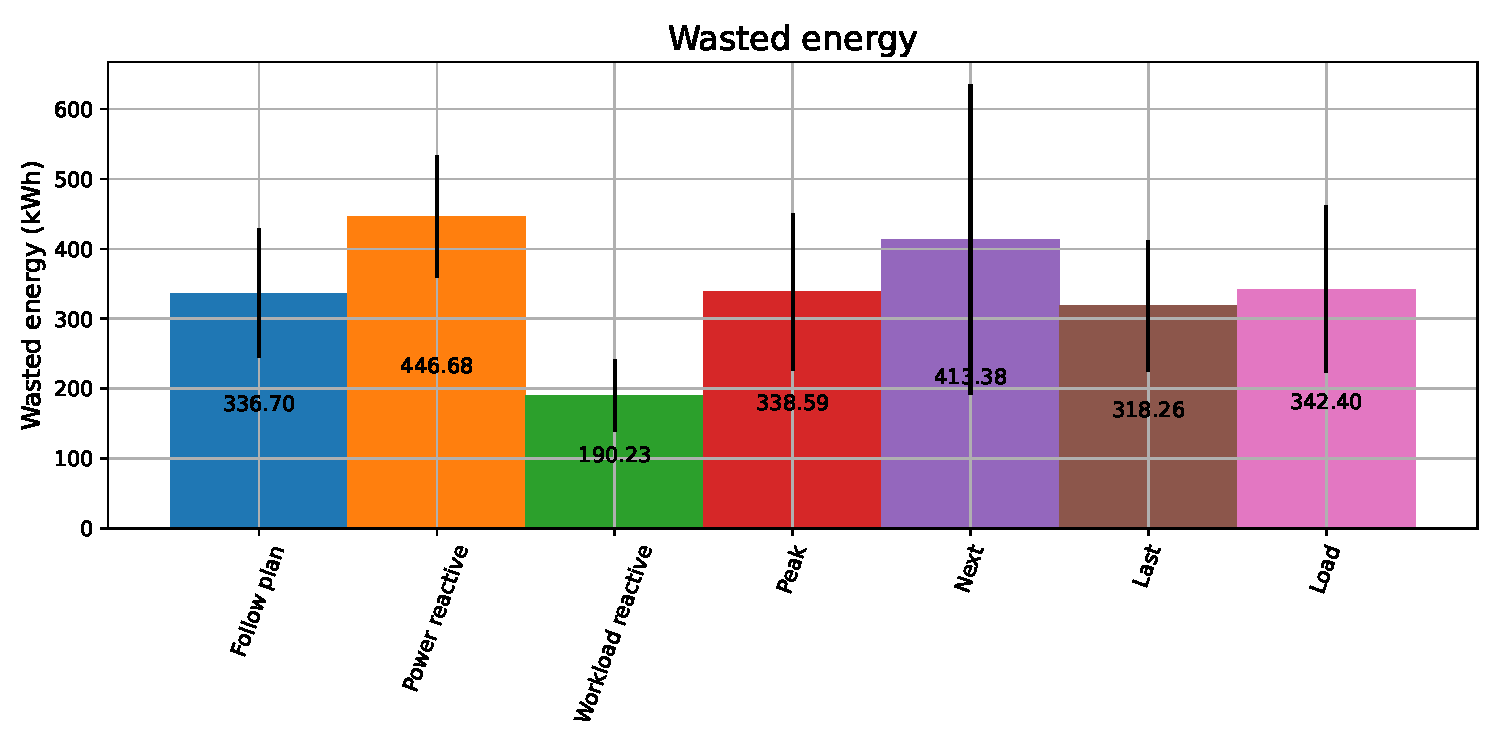
\includegraphics[scale=0.55]{Images/Compensations/energy_diff.pdf}
    \caption{Wasted energy at 100 random cases.}
    \label{fig:energy_diff}
\end{figure}

\clearpage

\subsection{Discussion}
\label{sec:compensation_discussion}

After presenting all results, this section discusses them generally. We highlight the advantages and disadvantages of all algorithms. Finally, we detail the gaps in the four policies that the following sections explore. The first algorithm is \emph{Follow plan}. This algorithm does not react to real events, applying the offline plan with no modifications. The results show that this approach tends to kill big jobs. Since the workload is composed of several small jobs (see Figure \ref{fig:metacentrum}), it can finish several jobs by number but not so much considering their size. Figure \ref{fig:jobs_critical_4} illustrates this case, where the algorithm finishes 85.48\% of jobs considering the number but only 57.70\% considering the size. This behavior also happens in random cases, where it finishes more than 90\% of the jobs in number but just more than 60\% in size (considering the median). Besides, \emph{Follow plan} does not use the surplus energy to run more jobs in scenarios 1 and 2. So, it saves energy but kills several jobs. This behavior can lead to highly wasted energy, like in critical scenario 1 (see Figure \ref{fig:energy_critical_1}). Since \emph{Follow plan} does not adjust the plan, it finishes with higher SoC in cases with higher energy and lower SoC with less energy. The 100 random cases show that the minimal value is close to -20\% and the maximum value is above 30\%. These results highlight the importance of plan adaptations.

Then, a question comes up: Why not use fully reactive algorithms? Then, we presented \emph{Power reactive} and \emph{Workload reactive}. \emph{Power reactive} adapts the servers' speed according to the power available from renewable. It uses the battery to maintain a server available if the incoming renewable production is not enough. \emph{Power reactive} finishes with a very low battery level, even in scenarios with more energy incoming from renewable. This algorithm only recharges the battery if the servers do not use the incoming renewable (e.g., a server stays idle). However, it is not enough. Another problem in \emph{Power reactive} is wasted energy. It has the worst results in every scenario. Since it does not use an offline plan, it wastes a lot of energy in transition states. For example, if renewable production is high, it will turn on several servers. Nevertheless, if the production drops in the next step, it turns them off. So, it wasted energy just reacting to the power available.

\emph{Workload reactive} is a very good algorithm from the QoS point of view. Considering the slowdown, for example, jobs do not wait too long to be placed. In addition, it can finish more jobs than the other algorithms. However, it can be too aggressive. It kills several jobs due to poor battery management in critical scenarios 1 and 3. Figure \ref{fig:DPM_soc} illustrates that \emph{Workload reactive} places all the incoming jobs on the first day, dropping the battery level too fast. When SoC arrives at 20\%, \emph{Workload reactive} turns off all servers, killing several jobs and increasing the slowdown. This also happens in critical scenario 3. In critical scenarios 2 and 4, it finishes with less battery level than the target. In random scenarios, the final battery level of \emph{Workload reactive} varies a lot, going from -30\% to more than 40\%. So, this algorithm has poor battery management, like \emph{Power reactive}. Even if it seems appropriate to use the battery to maximize the number of finished jobs, the next time window will not have energy in the batteries to use. Therefore, both reactive algorithms are not viable for a renewable-only data center.

So, we proposed four policies to adapt power usage, mixing the offline plan with reactiveness. \emph{Peak}, \emph{Next}, \emph{Last}, and \emph{Load} fulfill their main objective, approximating the battery level to the target level. In the profile worst-case scenarios (3 and 4), they degrade the QoS to approximate the battery level to the target. They do it by reducing power usage before the end of the time window. On the other hand, they use the surplus energy from scenarios with profile best-case (1 and 2) to run more jobs. In scenario 1, they are even better than the \emph{Workload reactive}. The policies finished very close to the target level in the random cases. To do so, they impact the total finished jobs but have a more controlled number of killed jobs than the baselines. For example, \emph{Last} never killed more than 12\% (in number). Therefore, these experiments show the impact on QoS of respecting the battery level.

It is hard to indicate the best policy. \emph{Last} policy is the best one in critical scenarios 1 and 2. It finishes more jobs in number and size in critical scenario 1 and the second best in critical scenario 2. These scenarios have more energy, so \emph{Last} puts the positive compensations in the last step. When it needs more energy to maintain servers running, it takes the energy from the same step. So, it is more likely for \emph{Last} to use the surplus energy. The drawback of the \emph{Last} policy is that the last step can be too late to use the energy (see Figure \ref{fig:SoC_critical_1}), and it can miss opportunities to turn on servers to run more jobs. For example, \emph{Load} has a better slowdown than \emph{Last} in critical scenario 1 (see Figure \ref{fig:slowdown_critical_1}). \emph{Load} turns on servers in the moments where they are needed. So, when the jobs arrive, servers are waiting for them. \emph{Load} is the second best in scenarios 1 and 2. With more energy, it puts energy in the steps with a higher deficit between production and demand. However, the prediction is not perfect. So, \emph{Load} can improve the wrong step. \emph{Next} has the worst results in these scenarios because it uses the surplus as soon as possible. Therefore, \emph{Next} makes it difficult to find energy in future steps to avoid killing jobs. Finally, \emph{Peak} has a balanced result in scenarios 1 and 2. It tends to maintain a more constant number of servers available over the steps. 

Regarding critical scenario 3, \emph{Next} and \emph{Peak} are good. This scenario has less energy available. Therefore, \emph{Next} adapts as soon as possible the usage. \emph{Peak} reduces the usage peak, maintaining a more stable usage. The behavior of both policies helps to avoid the lower battery boundary without starting too many jobs that can not be finished. \emph{Load} is too aggressive here, dropping the SoC too fast and killing several jobs. Here, \emph{Last} is not so good. It does not adapt the usage on the first day, arriving faster at SoC lower boundary. In the last critical scenario, \emph{Peak} is the best among the policies. It has the lowest killed jobs (in number and size). \emph{Next} has a good number of finished jobs, but a high number of killed jobs. Considering the size, it has the worst percentage of finished jobs. \emph{Load} is still aggressive, finishing fewer jobs (in number). \emph{Last} is a little better in this critical scenario, compared to the previous one. However, it still kills several jobs (second-worst among the policies). 

Finally, considering the 100 random cases, \emph{Last} finishes more jobs in number and size. \emph{Peak} and \emph{Load} are close, with \emph{Next} being the worst one. Comparing killed jobs, \emph{Last} and \emph{Peak} killed fewer jobs than \emph{Next} and \emph{Load}. \emph{Load} is too aggressive, and \emph{Next} compensates too soon. 

Considering all these results, we can say that: 
\begin{enumerate}
    \item \emph{Last} policy is the best one when we have more power arriving. Letting the power in the end, helps to migrate a second time when needed. However, it can miss the opportunities to turn on more servers in demand peak;
    \item \emph{Peak} policy has a good overall result, independent of the power profile;
    \item \emph{Next} policy is good in a context where the production is lower, and the demand peak is on the first day. In this scenario, the SoC drops too fast, and \emph{Next} adapts the usage sooner than the other policies;
    \item \emph{Load} policy is aggressive, which improves slowdown but can lead to several killed jobs.
\end{enumerate}

Regarding wasted energy, \emph{Next} is more likely to waste more than the other policies. It reintroduces the surplus as soon as possible, even if it is not necessary. \emph{Last} uses the energy wisely, since it places at the end, using before if necessary. \emph{Peak} and \emph{Load} depend on the scenario. Then, a new question comes up: is it possible to improve the Quality of Service in these scenarios, while still respecting the battery level at the end of the time window? To do so, the next chapter tries to mix the policies. For example, we can use \emph{Load} for some positive compensations to improve QoS, then use \emph{Last} for the remaining energy surplus. We proposed a model using reinforcement learning to find out which policy to use at each moment.

\section{Conclusion}
This chapter proposed new heuristics to approximate the battery storage level to the target level. These heuristics use surplus energy to improve the QoS, mainly the finished jobs. The policies try to reduce the impact on QoS in scenarios with less energy. The following chapter takes a step further, trying to mix the policies and improving QoS even more.